\documentclass[letterpaper, 11pt, oneside]{book}

\usepackage{style}  % If you feel like procrastinating, mess with this file
\usepackage{algo}   % Thank you Jeff, very cool!

\addbibresource{refs.bib}

% Required reading
% https://jmlr.csail.mit.edu/reviewing-papers/knuth_mathematical_writing.pdf
%   Along with required viewing:
%   https://www.youtube.com/watch?v=N6QEgbPWUrg&list=PLOdeqCXq1tXihn5KmyB2YTOqgxaUkcNYG
% https://faculty.math.illinois.edu/~west/grammar.html

% % % % % % % % % %
%     Cursor      %
%     Parking     %
%     Lot         %
% % % % % % % % % %

% Disable check for mismatched parens/brackets/braces
%   chktex-file 9
% Disable check for different counts of parents/brackets/braces
%   chktex-file 17
% Exclude these environments from syntax checking
%   VerbEnvir { tikzcd }

\regtotcounter{figure}

\title{\vspace{-100pt} {\Huge Using Algebraic Geometry} \\ {\small With $\total{figure}$ Figures}}
\author{\Large Anakin Dey}
\DTMsavenow{now}
\date{\small Last Edited on \today\ at \DTMfetchhour{now}:\DTMfetchminute{now}}

% Cover page number chicanery
\newcommand{\CoverName}{Cover}

\begin{document}
\frontmatter
\renewcommand{\thepage}{\CoverName}
\maketitle

\pagenumbering{roman}

\tableofcontents
\clearpage


% \listoftheorems[ignoreall, show={defn}, title={List of Definitions}]
%
% \listoftheorems[ignoreall, show={ex}, title={List of Examples and Counterexamples}]

\chapter*{Preface}

At the time of writing this, I am starting my PhD at The Ohio State University.
Currently a large part of my interests in algebra are about algorithms as they relate to polynomials and algebraic geometry.
I've been doing a bunch of problems from \emph{Ideals, Varieties, and Algorithms}~\cite{book:IVA}.
However,  it seems that \emph{Using Algebraic Geometry}~\cite{book:UAG} moves through the material faster as it assumes you know more algebra.
So I've moved onto working through this book as well as trying to comprehend Sturmfel's \emph{Algorithms in Invariant Theory}~\cite{book:AlgosInInvTheory}.

\mainmatter

\chapter{Introduction}

\section{Polynomials and Ideals}

\begin{sol}[\cite{book:UAG} Ex. 1.1.1]\label{ex:UAG_1.1.1}
  \begin{enumerate}
    \item We have that $x(x - y^{2}) + y(xy) = x^{2} - xy^{2} + xy^{2} = x^{2}$.
    \item It suffices to check for generators.
          We have that $x + (-1)(y^{2}) = x - y^{2}, y(x) = xy$, and $y^{2} = y^{2}$ showing that $\ideal{x - y^{2}, xy, y^{2}} \subseteq \ideal{x, y^{2}}$.
          Then $x - y^{2} + y^{2} = x$ and $y^{2} = y^{2}$ shows the reverse containment and overall the ideals are equal.
    \item We already know from 1.\ that $x^{2}$ lives in $\ideal{x - y^{2}, xy}$.
          Since $xy = xy$, we overall have that $\ideal{x^{2}, xy} \subseteq \ideal{x - y^{2}, xy}$.
          It remains to check if $x - y^{2} \in \ideal{x^{2}, xy}$.
          However, notice that every element of $\ideal{x^{2}, xy}$ is divisible by $x$ while $x - y^{2}$ is clearly not divisible by $x$.
          Thus $x - y^{2} \notin \ideal{x^{2}, xy}$ and the two ideals are not equal.
  \end{enumerate}
\end{sol}

\begin{sol}[\cite{book:UAG} Ex. 1.1.2]\label{ex:UAG_1.1.2}
  Let $f, g \in \ideal{f_{1}, \ldots, f_{s}}$.
  Then $\exists p_{1}, \ldots, p_{s}, q_{1}, \ldots, q_{s}$ such that $f = \sum_{i = 1}^{s} p_{i} \cdot f_{i}$ and $g = \sum_{i = 1}^{s} q_{i} \cdot f_{i}$.
  Thus $f + g = \sum_{i = 1}^{s} (p_{i} + q_{i}) \cdot f_{i}$ which shows that $f + g \in \ideal{f_{1}, \ldots, f_{s}}$.
  Then let $p \in k[x_{1}, \ldots, x_{n}]$.
  We have that $p \cdot f = p\sum_{i = 1}^{s} p_{i} f_{i} = \sum_{i = 1}^{s} (p \cdot p_{i}) \cdot f_{i}$ which shows that $\ideal{f_{1}, \ldots, f_{s}}$ is an ideal.
\end{sol}

\begin{sol}[\cite{book:UAG} Ex. 1.1.3]\label{ex:UAG_1.1.3}
  We already know that $\ideal{f_{1}, \ldots, f_{s}}$ is an ideal by \nameref{ex:UAG_1.1.2}.
  Now suppose that $J$ is an ideal containing $\set{f_{1}, \ldots, f_{s}}$.
  Then, since ideals are closed under addition and scaling, we have that for all $p_{1}, \ldots, p_{s} \in k[x_{1}, \ldots, x_{n}]$ that $\sum_{i = 1}^{s} p_{i} \cdot f_{i} \in J$.
  Thus, $\ideal{f_{1}, \ldots, f_{s}} \subseteq J$.
\end{sol}

\begin{sol}[\cite{book:UAG} Ex. 1.1.4]\label{ex:UAG_1.1.4}
  We claim that $\ideal{f_{1}, \ldots, f_{s}} = \ideal{g_{1}, \ldots, g_{t}}$ if and only if $\set{g_{1}, \ldots, g_{t}} \subseteq I$ and $\set{f_{1}, \ldots, f_{s}} \subseteq J$.
  The forward implication is immediate.
  Then by \nameref{ex:UAG_1.1.3}, if $\set{g_{1}, \ldots, g_{t}} \subseteq I$ then $J \subseteq I$.
  Similarly, $\set{f_{1}, \ldots, f_{s}} \subseteq J \implies I \subseteq J$ and overall $I = J$.
  This fact was used in \nameref{ex:UAG_1.1.1} (b).
\end{sol}

\begin{sol}[\cite{book:UAG} Ex. 1.1.5]\label{ex:UAG_1.1.5}
  It suffices to show that $z - x^{3} \in \ideal{y - x^{2}, z - xy}$ and and $z - xy \in \ideal{x - y^{2}, z - x^{3}}$.
  Indeed we have that $(z - xy) + x(y - x^{2}) = z - x^{3}$ which also yields that $z - xy = z - x^{3} - x(y - x^{2})$.
\end{sol}

\begin{sol}[\cite{book:UAG} Ex. 1.1.6]\label{ex:UAG_1.1.6}
  If $I = \set{0}$ then $I = \ideal{0}$.
  So suppose $I \neq 0$.
  Let $d \in I$ be of minimal degree.
  \quest{$d = \gcd(I)$ but I need infinite Bezout.}
  Then we claim that $\ideal{d} = I$.
  Since $d \in I$, we have that $\ideal{d} \subseteq I$.
  Now let $f \in I$.
  By Euclidean division, there exists $q, r \in k[x]$ such that $f = qd + r$ where either $r = 0$ or $0 \leq \deg(r) \leq \deg(d) - 1$.
  If $r = 0$ then $f \in \ideal{d}$ and we are done.
  So suppose $r \neq 0$.
  Then $f, qd \in I \implies r = f - qd \in I$.
  Thus, $r \in I$ is of degree strictly less than $d$, contradicting the minimality of the degree of $d$.
  So we must have that $r = 0$ and overall $\ideal{d} = I$.
\end{sol}

\begin{sol}[\cite{book:UAG} Ex. 1.1.7]\label{ex:UAG_1.1.7}
  \begin{enumerate}
    \item Suppose $f(x) \in \ideal{x}$.
          Then $f(x)^{m} \in \ideal{x^{n}}$ so $f(x) \in \sqrt{\ideal{x^{n}}}$
          Now suppose that $f(x) \in \sqrt{\ideal{x^{n}}}$.
          Then $\exists k$ such that $f(x)^{k} \in \ideal{x^{n}}$.
          Thus $f(x)^{k}$ is a multiple of $x^{n}$.
          This implies that $f(x)^{k}$ is a multiple of $x$.
          Then notice that the unique factorization of $f(x)^{k}$ into irreducibles is the $k$th power of the factorization of $f(x)$ into irreducibles.
          Thus $x$ must be a factor of $f(x)$ and so $f(x) \in \ideal{x}$.
          Note, this heavily uses the fact that $k[x]$ is a unique factorization domain for all fields $k$.
    \item We claim that $\sqrt{\ideal{p(x)}} = \ideal{(x - a_{1}) \cdots (x - a_{m})} = I$.
          Suppose $f(x) \in I$.
          Let $k = \max{e_{1}, \ldots, e_{n}}$.
          Then $p(x) \mid f(x)^{k}$ so $f(x) \in \sqrt{\ideal{p(x)}}$.
          Now suppose that $f(x) \in \sqrt{\ideal{p(x)}}$.
          Then $\exists k$ such that $f(x)^{k} \in \ideal{p(x)}$.
          Thus $f(x)^{k}$ is a multiple of each $(x - a_{i})$.
          Then notice that the unique factorization of $f(x)^{k}$ into irreducibles is the $k$th power of the factorization of $f(x)$ into irreducibles.
          Thus $f(x)$ is a multiple of each $(x - a_{i})$ and so $f(x) \in I$.
    \item Radical ideals are the ideals $I$ such that $\sqrt{I} = I$.
          Notice that $\C[x]$ is a principal ideal domain and so any such $I$ must be generated by a single polynomial.
          Since every polynomial in $\C[x]$ splits into linear factors, (b) immediately implies that the only radical ideals of $\C[x]$ are the ones which are of the form $\ideal{(x - a_{1}) \cdots (x - a_{m})}$ for $a_{1}, \ldots, a_{m} \in \C[x]$.
  \end{enumerate}
\end{sol}

\clearpage

\begin{sol}[\cite{book:UAG} Ex. 1.1.8]\label{ex:UAG_1.1.8}
  \begin{enumerate}
    \item Let $\mathfrak{p}$ be a prime ideal in $k[\overline{x}]$.
          Clearly $\mathfrak{p} \subseteq \sqrt{\mathfrak{p}}$ always.
          Let $f(\overline{x}) \in \sqrt{\mathfrak{p}}$.
          Then $f(\overline{x})^{m} \in \mathfrak{p}$ for some $m \in \Z_{\geq 1}$.
          We prove the reverse inclusion by induction on $m$.
          If $m = 1$ then $f(\overline{x}) =f(\overline{x})^{1} \in \mathfrak{p}$.
          Now let $m > 1$ and suppose the claim holds for all $k \leq m$.
          Then suppose $f(\overline{x})^{m + 1} \in \mathfrak{p}$.
          Then $f(\overline{x}) \cdot f(\overline{x})^{m} \in \mathfrak{p}$/
          Either $f(\overline{x}) \in \mathfrak{p}$ or $f(\overline{x})^{m} \in \mathfrak{p}$ which by induction implies that $f(\overline{x}) \in \mathfrak{p}$.
          Thus, $f(\overline{x})^{m} \in \mathfrak{p} \implies f(\overline{x}) \in \mathfrak{p}$ for all $m \in \Z_{\geq 1}$ and so $\sqrt{\mathfrak{p}} \subseteq \mathfrak{p}$.
          Thus, all prime ideals are radical.
    \item Notice that for all fields $k$ that $k[x]$ is a principal ideal domain.
          Thus, all the prime ideals are the ones generated by a single irreducible polynomial.
          Also, in $k[x]$ we have that $(0)$ is a prime ideal as well as $k[x]$ is an integral domain.
          In $\C[x]$, these are the ideals generated by $x - z$ for some $z \in \C$.
          In $\R[x]$, the primes are the ideals generated by $x - r$ for some $r \in \R$ or $x^{2} + r$ for some positive $r \in R$.
          \quest{What would be a general condition for $\Q[x]$?}
  \end{enumerate}
\end{sol}

\begin{sol}[\cite{book:UAG} Ex. 1.1.9]\label{ex:UAG_1.1.9}
  \begin{enumerate}
    \item First, observe that $\ideal{x_{1}, \ldots, x_{n}}$ is the ideal consisting exactly of polynomials which have no constant term.
          Let $I$ be an ideal in $k[x_{1}, \ldots, x_{n}]$ such that $\ideal{x_{1}, \ldots, x_{n}} \subsetneq I$.
          Thus there exists $f(x_{1}, \ldots, x_{n}) \in I \setminus \ideal{x_{1}, \ldots, x_{n}}$.
          We have by our observation that $f$ has a nonzero constant term $z$.
          Then note that the non-constant terms of $f$ form a polynomial $g(x_{1}, \ldots, x_{n})$ in $\ideal{x_{1}, \ldots, x_{n}}$.
          Thus, we have that $z = f(x) - g(x) \in I$.
          Since $I$ contains a nonzero constant term, we must have that $I = k[x_{1}, \ldots, x_{n}]$.
    \item Recall that an ideal $I$ is maximal if and only if $R/I$ is a field.
          Let $I = \ideal{x_{1} - a_{1}, \ldots, x_{n} - a_{n}}$.
          Consider the evaluation map $\text{ev}_{\overline{a}}\colon k[x_{1}, \ldots, x_{n}] \to k$ sending $f(x_{1}, \ldots, x_{n}) \mapsto f(a_{1}, \ldots, a_{n})$.
          Clearly this map is surjective.
          Then since for all $i$ we have that $x_{i} \equiv a_{i} \pmod{I}$, we have that $f(x_{1}, \ldots, x_{n}) \equiv f(a_{1}, \ldots, a_{n}) \pmod{I}$ for all $f(x_{1}, \ldots, x_{n}) \in k[x_{1}, \ldots, x_{n}]$.
          Thus, $\text{ev}_{\overline{a}}(f) = f(a_{1}, \ldots, a_{n}) = 0$ if and only if $f(x_{1}, \ldots, x_{n}) \in I$.
          Thus, $\ker(\text{ev}_{\overline{a}}) = I$ and $k[x_{1}, \ldots, x_{n}] / I$ is a field, meaning $\ideal{x_{1} - a_{1}, \ldots, x_{n} - a_{n}}$ is maximal.
    \item Since $\R[x]$ is a principal ideal domain, any ideal $I$ strictly containing $\ideal{x^{2} + 1}$ is of the form $\ideal{g(x)}$ for some $g(x) \mid x^{2} + 1$.
          However, since $x^{2} + 1$ is irreducible in $\R[x]$, we have that $g(x)$ is either $z(x^{2} + 1)$ for some nonzero $z \in \C$ or $g(x) = z$ for some nonzero $z \in \C$, meaning $\ideal{g(x)} = \ideal{x^{2} + 1}$ or or $\ideal{g(x)} = \R[x]$.
          Thus, $\ideal{x^{2} + 1}$ is maximal.
          However, in $\C[x]$, we have that $x^{2} + 1 = (x + i)(x - i)$ and so $\ideal{x^{2} + 1} \subsetneq \ideal{x - i} \subsetneq \C[x]$.
  \end{enumerate}
\end{sol}

\clearpage

\begin{sol}[\cite{book:UAG} Ex. 1.1.10]\label{ex:UAG_1.1.10}
  \begin{enumerate}
    \item Since $x^{2} + y^{2} - (x^{2} - z^{3}) = y^{2} + z^{3}$ is an element of $I$ which does not depend on $x$, $y^{2} + z^{3}$ is in $I_{1}$.
    \item For all $\ell \geq 1$, we have that $0 \in I_{\ell}$.
          Then, if $f(x_{\ell + 1}, \ldots, x_{n}), g(x_{\ell + 1}, \ldots, x_{n})$ are two polynomials in $I$ who do not depend on the first $\ell$ variables, then so is $f + g$.
          Finally, let $r(x_{\ell} + 1, \ldots, x_{n}) \in k[x_{\ell + 1}, \ldots, x_{n}]$.
          Then $r \cdot f \in I_{\ell}$ since $r \cdot f \in I$ and still does not depend on any of the first $\ell$ variables.
  \end{enumerate}
\end{sol}

\begin{sol}[\cite{book:UAG} Ex. 1.1.11]\label{ex:UAG_1.1.11}
  \begin{enumerate}
    \item \quest{meh}
    \item \quest{meh}
    \item We claim that $I + J = \ideal{f_{1}, \ldots, f_{s}, g_{1}, \ldots, g_{t}}$.
          Clearly $I, J \subseteq \ideal{f_{1}, \ldots, f_{s}, g_{1}, \ldots, g_{t}}$ and thus so is $I \cup J$.
          By (b), this shows that $I + J \subseteq \ideal{f_{1}, \ldots, f_{s}, g_{1}, \ldots, g_{t}}$.
          Then, since $f_{i} = f_{i} + 0$ and $g_{j} = 0 + g_{j}$ for all $i, j$, we have the reverse inclusion and thus the two ideals are equal.
  \end{enumerate}
\end{sol}

\begin{sol}[\cite{book:UAG} Ex. 1.1.12]\label{ex:UAG_1.1.12}
  \begin{enumerate}
    \item \quest{meh}
    \item Suppose that $h(\overline{x}) \in IJ$.
          Note that $IJ$ is generated by the products $f(\overline{x}) \cdot g(\overline{x})$ for $f(\overline{x}) \in I$, and $g(\overline{x}) \in J$.
          Then $h(\overline{x})$ consists of sums of terms of the form $r(\overline{x}) \cdot f(\overline{x}) \cdot g(\overline{x})$ for $r(\overline{x}) \in k[\overline{x}]$, $f(\overline{x}) \in I$, and $g(\overline{x}) \in J$.
          Thus, each term is in both $I$ and $J$ and overall so is $h(\overline{x})$.

          To see an example where $IJ \subsetneq I \cap J$, consider $I = \ideal{x^{2}y}$ and $J = \ideal{xy^{2}}$ in $k[x, y]$.
          Then $I \cap J = \gen{x^{2}y^{2}}$ and $IJ = \gen{x^{3}y^{3}}$.
          Thus $IJ \subsetneq I \cap J$ as $I \cap J$ contains $x^{2}y^{2}$ and $IJ$ does not contain $x^{2}y^{2}$.
  \end{enumerate}
\end{sol}

\clearpage

\section{\Grobner\ Bases}

\begin{sol}[\quest{\cite{book:UAG} Ex. 1.3.11}]\label{ex:UAG_1.3.11}

\end{sol}

\clearpage

\section{Affine Varieties}

\begin{sol}[\quest{\cite{book:UAG} Ex. 1.4.9}]\label{ex:UAG_1.4.9}

\end{sol}

\chapter{Solving Polynomial Equations}

\section{Solving Polynomial Systems by Elimination}

\begin{sol}[\quest{\cite{book:UAG} Ex. 2.1.1}]\label{ex:UAG_2.1.1}

\end{sol}

\begin{sol}[\quest{\cite{book:UAG} Ex. 2.1.2}]\label{ex:UAG_2.1.2}

\end{sol}

\begin{sol}[\cite{book:UAG} Ex. 2.1.3]\label{ex:UAG_2.1.3}
  We may freely rewrite the polynomial as $p(z) = z^{n} - a_{n - 1}z^{n - 1} - \cdots - a_{0}$
  We have that $0 = \overline{z}^{n} - a_{n - 1}\overline{z}^{n - 1} - \cdots - a_{0}$ and so $\overline{z}^{n} = a_{n - 1}\overline{z}^{n - 1} + \cdots + a_{0}$.
  Suppose now that $\abs{\overline{z}} \geq 1$.
  Then
  \[
    \abs{\overline{z}}^{n} = \abs{a_{n - 1}\overline{z}^{n - 1} + \cdots + a_{0}} \leq \abs{a_{n - 1}}\abs{z}^{n - 1} + \cdots + a_{0} \leq \abs{a_{n - 1}}\overline{z}^{n - 1} + \cdots \abs{a_{0}}\overline{z}^{n - 1}.
  \]
  Thus, $\abs{\overline{z}} \leq \abs{a_{n - 1}} + \cdots + \abs{a_{0}}$.
  However, we assumed that $\abs{\overline{z}} \geq 1$.
  This may not be the case.
  Thus, $\abs{\overline{z}} \leq B \defeq \max\set{1, \abs{a_{n - 1}} + \cdots + \abs{a_{0}}}$.
\end{sol}

\begin{sol}[\quest{\cite{book:UAG} Ex. 2.1.4}]\label{ex:UAG_2.1.4}
  Numerically find all roots of $2z^{6} + 2z^{5} - z^{4} - z^{3} - 2z^{2} - 2z - 2$.
\end{sol}

\clearpage

\begin{sol}[\cite{book:UAG} Ex. 2.1.5]\label{ex:UAG_2.1.5}
  We apply Buchberger's Criterion.
  Let $f(x, y) = x^{2} + 2x + 3 + y^{5} - y$ and $g(x, y) = y^{6} - y^{2} + 2y$.
  Then we have that
  \[
    S(f, g) = \frac{x^{2}y^{6}}{x^{2}} \cdot (x^{2} + 2x + 3 + y^{5} - y) - \frac{x^{2}y^{6}}{y^{6}} \cdot (y^{6} - y^{2} + 2y) = y^{6} \cdot (x^{2} + 2x + 3 + y^{5} - y) - x^{2} \cdot (y^{6} - y^{2} + 2y).
  \]
  This shows that $\overline{S(f, g)}^{G} = 0$ which yields that $G$ is a \Grobner\ basis.
\end{sol}

\begin{sol}[\quest{\cite{book:UAG} Ex. 2.1.6}]\label{ex:UAG_2.1.6}
\end{sol}

\begin{sol}[\quest{\cite{book:UAG} Ex. 2.1.7}]\label{ex:UAG_2.1.7}
\end{sol}

\clearpage

\begin{sol}[\cite{book:UAG} Ex. 2.1.8]\label{ex:UAG_2.1.8}
  \begin{enumerate}
    \item Let $\overline{z}$ be a simple root of $p(z)$, so $p(z) = 0$ but $p'(z) \neq 0$.
          Then $N_{p}(\overline{z}) = \overline{z} - \frac{p(\overline{z})}{p'(\overline{z})} = \overline{z}$ meaning $\overline{z}$ is a fixed point of $N_{p}(z)$.
    \item Suppose that $\overline{z}$ is a multiple root of $p(z)$ with multiplicity $m \geq 2$.
          Then we may express $p(z) = \tilde(p)(z)(z - \overline{z})^{m}$ such that $\tilde{p}(\overline{z}) \neq 0$.
          Thus, we have that
          \begin{align*}
            N_{p}(z) &\defeq z - \frac{p(z)}{p'(z)} \\
            &= z - \frac{\tilde{p}(z)(z - \overline{z})^{m}}{\tilde{p}'(z)(z - \overline{z})^{m} + m\tilde{p}(z)(z - \overline{z})^{m - 1}} = z - \frac{\tilde{p}(z)(z - \overline{z})}{\tilde{p}'(z)(z - \overline{z}) + m\tilde{p}(z)}
          \end{align*}
          Note that $m\tilde{p}(\overline{z}) \neq 0$.
          Thus, we have that
          \[
            \abs{N_{p}(\overline{z})} = \abs{\overline{z} - \frac{\tilde{p}(\overline{z})(\overline{z} - \overline{z})}{\tilde{p}'(\overline{z})(\overline{z} - \overline{z}) + m\tilde{p}(\overline{z})}} = \abs{\overline{z}} \leq \lc(p) \cdot B
          \]
          where $B$ is the value from~\nameref{ex:UAG_2.1.3} and $\lc(p)$ is the leading coefficient of $p(z)$.
    \item Suppose now that $\overline{z}$ is a simple root of $p(\overline{z})$.
          Then we may express $p(z) = \tilde{p}(z)(z - \overline{z})$ such that $\tilde{p}(\overline{z}) \neq 0$.
          We have that
          \[
            p'(z) = \tilde{p}'(z)(z - \overline{z}) + \tilde{p}(z)
          \]
          and evaluation of $p'(z)$ at $\overline{z}$ is nonzero.
    \item Let $\overline{z}$ be a root of multiplicity $m$.
          Following (b), we write $p(z) = \tilde{p}(z)(z - \overline{z})^{m}$ such that $\tilde{p}(\overline{z}) \neq 0$.
          Then we have, by differentiating the expression for $N_{p}(z)$ from (b), that
          \[
            N'_{p}(z) = 1 - \frac{(\tilde{p}'(z)(z - \overline{z}) + \tilde{p}(z))(\tilde{p}'(z)(z - \overline{z}) + m\tilde{p}(z)) - (\tilde{p}(z)(z - \tilde{z}))(\tilde{p}''(z)(z - \overline{z}) + \tilde{p}'(z) + m\tilde{p}'(z))}{(\tilde{p}'(z)(z - \overline{z}) + m\tilde{p}(z))^{2}}.
          \]
          Evaluation at $z = \overline{z}$ yields that $\lim_{z \to \overline{z}} N_{p}'(z) = 1 - \frac{1}{m}$.
    \item Let $\overline{z}$ be a root of multiplicity $m$.
          Following (b), we write $p(z) = \tilde{p}(z)(z - \overline{z})^{m}$ such that $\tilde{p}(\overline{z}) \neq 0$.
          Then
          \[
            p'(z) = \tilde{p}'(z - \overline{z})^{m} + m\tilde{p}(z)(z - \overline{z})^{m - 1} = (z - \overline{z})^{m - 1}(\tilde{p}'(z)(z - \overline{z}) + m\tilde{p}(z)).
          \]
          Notice that $\tilde{p}'(\overline{z})(\overline{z} - \overline{z}) + m\tilde{p}(\overline{z}) = m\tilde{p}(\overline{z}) \neq 0$.
          Thus, a root of multiplicity $m \geq 1$ of $p(z)$ is a root of multiplicity $m - 1$ of $p'(z)$.
          This implies that if we have roots $\overline{z}_{1}, \ldots, \overline{z}_{k}$ with multiplicities $m_{1}, \ldots, m_{k} \geq 1$, then $\gcd(p(z), p'(z)) = (z - \overline{z}_{1})^{m_{1}} \cdots (z - \overline{z}_{k})^{m_{k}}$.
          Thus, the polynomial $p_{\mathrm{red}}(z) = \frac{p(z)}{\gcd(p(z), p'(z))}$ has the same roots of $p(z)$ but all with multiplicity $1$ which is the best case for Newton's method.
  \end{enumerate}
\end{sol}

\begin{sol}[\cite{book:UAG} Ex. 2.1.9]\label{ex:UAG_2.1.9}
  \begin{enumerate}
    \item Let $p(z) = z^{2} + 1$.
          We have that
          \[
            N_{p}(z) = z - \frac{z^{2} + 1}{2z} = \frac{2z^{2} - z^{2} + 1}{2z} = \frac{z^{2} + 1}{2z} = \frac{x^{2} + 2ixy - y^{2} + 1}{2x + 2iy}.
          \]
          If $z$ is real then $y = 0$ and so $N_{p}(x) = \frac{x^{2} + 1}{2x}$ which is always real.
          Thus, Newton's method will never reach the imaginary roots of $z^{2} + 1$.
          However, if we begin with a guess with nonzero imaginary part, then the guess does converge as expected.
    \item \quest{Just basic arithmetic not worth doing.}
  \end{enumerate}
\end{sol}

\begin{sol}[\cite{book:UAG} Ex. 2.1.10]\label{ex:UAG_2.1.10}
  Let $\overline{z}$ be a root of $p(z)$.
  Then $-\overline{z}^{n} = a_{n - 1}\overline{z}^{n - 1} + \cdots + a_{0}$ and so
  \begin{align*}
    \abs{\overline{z}}^{n} &= \abs{a_{n - 1}\overline{z}^{n - 1} + \cdots + a_{0}} \\
                           &\leq \max_{i}\set{\abs{a_{i}}} \cdot \abs{\overline{z}^{n - 1} + \cdots + 1} \\
                           &\leq \max_{i}\set{\abs{a_{i}}} \cdot \pqty{\abs{\overline{z}}^{n - 1} + \cdots + 1} \\
                           &= \max_{i}\set{\abs{a_{i}}} \cdot \frac{\abs{\overline{z}}^{n} + 1}{\abs{\overline{z}} - 1} \leq \max_{i}\set{\abs{a_{i}}} \cdot \frac{\abs{\overline{z}}^{n}}{\abs{\overline{z}} - 1}.
  \end{align*}
  Thus, $\abs{\overline{z}}^{n} \leq \max_{i}\set{\abs{a_{i}}} \cdot \frac{\abs{z}^{n}}{\abs{z} - 1}$ which implies that $\abs{z} - 1 \leq \max_{i}\set{\abs{a_{i}}}$.
  Thus, $\abs{z} \leq 1 + \max_{i}\set{\abs{a_{i}}}$.
\end{sol}

\clearpage

\section{Finite Dimensional Algebras}

\begin{sol}[\quest{\cite{book:UAG} Ex. 2.2.1}]\label{ex:UAG_2.2.1}
\end{sol}

\begin{sol}[\cite{book:UAG} Ex. 2.2.2]\label{ex:UAG_2.2.2}
  It is clear that $\ideal{p_{i}(x_{i})} \subseteq I \cap k[x_{i}]$.
  Now suppose that $f(x_{i}) \in I \cap k[x_{i}]$.
  Then $\deg(f(x_{i}))$ must be $\geq m_{i}$.
  If not, then by the minimality of $m_{i}$ we would arrive at a contradiction.
  Now by the division algorithm, write $f(x_{i}) = q(x_{i})p_{i}(x_{i}) + r(x_{i})$ where $\deg(r_{x_{i}}) < m_{i}$.
  Then $r(x_{i}) = f(x_{i}) - q(x_{i})p(x_{i}) \in I$ and so $r(x_{i})$ must be $0$ since if not, we would arrive at a contradiction of the minimality of $m_{i}$.

  This gives us an algorithm to compute $p_{i}(x_{i})$.
  Let $I$ be a zero dimensional ideal and $G$ a \Grobner\ basis for $I$.
  Then we know there exists $m_{i}$ such that $\set{1, [x_{i}], \ldots, [x^{m_{i}}]}$ is linearly dependent in $k[\overline{x}] / I$.
  In fact, we may use the Finiteness Theorem to set $m_{i}$ to the smallest integer such that $x_{i}^{m_{i}} = \lt(g)$ for some $g \in G$.
  Since $k[x_{1}, \ldots, x_{n}] / I$ is a vector space, we can check linear independence in the usual way.
  See \texttt{code/ch2/2\_2\_2.sage} for a SageMath implementation of this.
\end{sol}

\begin{sol}[\cite{book:UAG} Ex. 2.2.3]\label{ex:UAG_2.2.3}
  Let $0 \neq f(x) \in \sqrt{\gen{p(x)}}$.
  Then there exists $m \geq 1$ such that $f^{m} \in \gen{p(x)}$ and so $p(x) \mid f(x)^{m}$.
  In particular, each linear factor $(x - \overline{z})$ of $p(x)$ divides $f(x)^{n}$ and so divides $f(x)$ as $(x - \overline{z})$ is irreducible.
  Thus, $p_{\red}(x) \mid f(x)$ and so $f(x) \in \gen{p_{\red}(x)}$.
  Conversely, suppose $f(x) \in \gen{p_{\red}(x)}$ so that $\gen{p_{\red}} \mid f(x)$.
  Label the roots of $p(x)$ as $\overline{z}_{1}, \ldots, \overline{z}_{r}$, each $\overline{z}_{i} \in \overline{k}$.
  Then for each $i$, $(x - \overline{z}_{i}) \mid f(x)$
  Let $m_{i}$ be the multiplicity of $z_{i}$ in $p(x)$ and $m = \max\set{m_{1}, \ldots, m_{r}}$.
  Then $p(x) \mid f(x)^{m}$ and so $f(x) \in \sqrt{\gen{p(x)}}$
\end{sol}

\begin{sol}[\cite{book:UAG} Ex. 2.2.4]\label{ex:UAG_2.2.4}
  We use the algorithm from \nameref{ex:UAG_2.2.2} implemented in \texttt{code/ch2/2\_2\_2sage}.
  See \texttt{code/ch2/2\_2\_2sage} for the code in action.
\end{sol}

\clearpage

\begin{sol}[\quest{\cite{book:UAG} Ex. 2.2.5}]\label{ex:UAG_2.2.5}
  Then $\sqrt{I} = I + \gen{x(x - 1), y(y - 2)}$.
  Since $I \subseteq \sqrt{I}$, we see that $\dim \C[x, y] / I \geq \dim \C[x, y] / \sqrt{I}$.
  A quick SageMath computation confirms this: $\dim \C[x, y] / I = 9$ and $\dim \C[x, y] / \sqrt{I} = 2$.
  See \texttt{code/ch2/2\_2\_5.sage} for the code in action.
  Then, since $I \subseteq \sqrt{I}$ we have that $V(\sqrt{I}) \subseteq V(I)$.
  Notice that
  \begin{align*}
    y^{4}x + 3x^{3} - y^{4} - 3x^{2} &= y^{4}(x - 1) + 3x^{2}(x - 1) = (y^{4} + 3x^{2})(x - 1) \\
    x^{2}y - 2x^{2} &= x^{2}(y - 2) \\
    2y^{4}x - x^{3} - 2y^{4} + x^{2} &= 2y^{4}(x - 1) - x^{2}(x - 1) = (2y^{4} - x^{2})(x - 1).
  \end{align*}
  Thus, $(1, 2)$ and $(0, 0)$ are the only two points in $V(I)$.
  Since it is evident that $V(\sqrt{I})$ contains these two points, we see in this case that $V(\sqrt{I}) = V(I)$.
\end{sol}

\begin{sol}[\cite{book:UAG} Ex. 2.2.6]\label{ex:UAG_2.2.6}
  A grevlex \Grobner\ basis for $I$ is $\set{y^{4} - 16y^{2}, x^{3} - x^{2}, -2x^{2}}$.
  Thus, by the Finiteness Theorem, we know that the for monomials $x^{a}y^{b}$ in $\C[x, y] / I$ we must have that $0 \leq a \leq 1$ and $0 \leq b \leq 3$.
  See \texttt{code/ch2/2\_2\_6.sage} for the code in action to compute the table.
\end{sol}

\begin{sol}[\cite{book:UAG} Ex. 2.2.7]\label{ex:UAG_2.2.7}
  We implement the algorithm described in \nameref{ex:UAG_1.3.11}.
  See \texttt{/code/ch2/2\_2\_7.sage} for the code in action.
\end{sol}

\begin{sol}[\cite{book:UAG} Ex. 2.2.8]\label{ex:UAG_2.2.8}
  \begin{enumerate}
    \item See \texttt{code/ch2/2\_2\_8.sage} for the code in action.
    \item Since each of the $I_{j}$ are maximal ideals and $I_{j} \subseteq \sqrt{I_{j}}$, we must have that $I = \sqrt{I_{j}}$.
          Thus $I(V(I_{j})) = I_{j}$ and we must have that $I_{j} = \sqrt{I_{j}}$.
          Since each $I_{j}$ is radical and $I = \bigcap_{j = 1}^{5} I_{j}$, we have by~\nameref{ex:UAG_2.2.7} that $I$ is radical.
  \end{enumerate}
\end{sol}

\clearpage

\begin{sol}[\cite{book:UAG} Ex. 2.2.9]\label{ex:UAG_2.2.9}
  \begin{enumerate}
    \item Let $f(\overline{x}) \in I + \ideal{p}$ and let $1 \leq j \leq d$.
          Then $f(\overline{x}) = g(\overline{x}) + h(\overline{x})p(x_{1})$ for some $g(\overline{x}) \in I$ and $h(\overline{x}) \in k[\overline{x}]$.
          We have that $(x_{1} - a_{j}) \mid p(x_{1})$ and so $h(\overline{x})p(x_{1}) \in \ideal{x_{1} - a_{j}}$.
          Thus, $f(\overline{x}) = g(\overline{x}) + h(\overline{x})p(x_{1}) \in I + \ideal{x_{1} - a_{j}}$.
          As $j$ was arbitrary, we have that $f(\overline{x}) \in \bigcap_{j} (I + \ideal{x_{1} - a_{j}})$.
    \item Let $f(\overline{x}) \in p_{j} \cdot (I + \ideal{x_{1} - a_{j}})$.
          Then $f(\overline{x}) = p_{j}(x_{1})\cdot(g(\overline{x}) + h(\overline{x})(x_{1} - a_{j}))$ for some $g(\overline{x}) \in I$ and $h(\overline{x}) \in k[\overline{x}]$.
          We have that $p_{j}(x_{1})g(\overline{x}) \in I$ and $p_{j}(x_{1})h(\overline{x})(x_{1} - a_{j}) = h(\overline{x})p(x_{1}) \in \ideal{p}$.
          Thus, $f(\overline(x)) = p_{j}(x_{1})g(\overline{x}) + h(\overline{x})p(x_{1}) \in I + \ideal{p}$.
    \item Let $d = \gcd(p_{1}, \ldots, p_{d})$.
          Then as $d \mid p_{1}$ and $d \mid p_{2}$, we have that $d \mid \prod_{j \neq 1, 2} (x_{1} - a_{j})$.
          Continuing on inductively, we have that for all $c \leq d$ that $d \mid \prod_{j \notin [c]} (x_{1} - a_{j})$.
          In particular, this means that $d \mid \prod_{j \notin [d]} (x_{1} - a_{j}) = 1$.
          Thus, $d$ itself is a unit in $k[\overline{x}]$ and $p_{i}$ and $p_{j}$ are coprime.
          By Bezout's Lemma, there exists polynomials $h_{1}, \ldots, h_{d} \in k[\overline{x}]$ such that $1 = \sum_{j = 1}^{d} h_{j}(\overline{x})p_{j}(x_{1})$.
    \item Now let $h(\overline{x}) \in \bigcap_{j = 1}^{d} (I + \ideal{x_{1} - a_{j}})$.
          As all the $p_{j}$ are coprime, we have that there exist polynomials $h_{1}, \ldots, h_{d} \in k[\overline{x}]$ such that $1 = \sum_{j = 1}^{d} h_{j}(\overline{x})p_{j}(x_{1})$.
          Thus, $h = \sum_{j = 1}^{d} h_{j}(\overline{x})p_{j}(x_{1})h(\overline{x})$.
          Then for all $1 \leq j \leq d$, we have that as $p_{j}(x_{1})h(\overline{x}) \in p_{j} \cdot (I + \ideal{x_{1} - a_{j}}) \subseteq I + \ideal{p}$.
          Thus, each summand of $\sum_{j = 1}^{d} h_{j}(\overline{x})p_{j}(x_{1})h(\overline{x})$ is in $I + \ideal{p}$ and so overall $h \in I + \ideal{p}$.
  \end{enumerate}
\end{sol}

\begin{sol}[\cite{book:UAG} Ex. 2.2.10]\label{ex:UAG_2.2.10}
  \begin{enumerate}
    \item Let $\overline{f}^{G} = \sum_{j = 1}^{d} c_{j}(f) x^{\alpha(j)}$ and $\overline{g}^{G} = \sum_{j = 1}^{d} c_{j}(g) x^{\alpha(j)}$.
          Then by combining like terms, we have that $\overline{f}^{G} + \overline{g}^{G} = \sum_{j = 1}^{d} (c_{j}(f) + c_{j}(g)) x^{\alpha(j)}$.
          On the other hand, we have that $\overline{f + g}^{G} = \sum_{j = 1}^{d} c_{j}(f + g) x^{\alpha(j)}$.
          Since $\overline{f}^{G} + \overline{g}^{G} = \overline{f + g}^{G}$ and each of the $x^{\alpha(j)}$ are linearly independent, we may equate coefficients and conclude that $c_{j}(f) + c_{j}(g) = c_{j}(f + g)$.
          For $\lambda \in k$, $\overline{\lambda f}^{G} = \sum_{j = 1}^{d} c_{j}(\lambda f) x^{\alpha(j)}$.
          Now notice that $\overline{\lambda f}^{G} = \lambda \overline{f}^{G}$ as we are working over a field.
          Thus, we have by equating coefficients that $c_{j}(\lambda f) = \lambda c_{j}(f)$.
          Thus, $c_{j}$ is a linear function $A \to k$.
    \item Let $\alpha_{j} \in A^{*}$ be the linear map $\alpha_{j}(f) = c_{j}(f)$.
          Notice that for all $1 \leq i, j \leq d$ we have that $\alpha_{j}(x^{\alpha(i)}) = c_{j}(x^{\alpha(i)}) = \delta_{i,j}$.
          Suppose there exists $\lambda_{1}, \ldots, \lambda_{d} \in k$ such that $\lambda_{1}\alpha_{1} + \cdots + \lambda_{d}\alpha_{d} = 0$.
          Then for all $1 \leq i \leq d$ we have that
          \[
            0 = \pqty{\sum_{j = 1}^{d} \lambda_{j} \alpha_{j}}(x^{\alpha(i)}) = \sum_{j = 1}^{d} \lambda_{j} \alpha_{j}(x^{\alpha(i)}) = \lambda_{i}
          \]
          and so for all $1 \leq i \leq d$, $\lambda_{i} = 0$ meaning that $\set{\alpha_{1}, \ldots, \alpha_{d}}$ is linearly independent.
          Since we know that $d = \dim A = \dim A^{*}$, we have that $\set{\alpha_{1}, \ldots, \alpha_{d}}$ is a basis for $A^{*}$.
    \item This was proven in \textbf{(b)}.
  \end{enumerate}
\end{sol}

\begin{sol}[\cite{book:UAG} Ex. 2.2.11]\label{ex:UAG_2.2.11}
  \begin{enumerate}
    \item We want a linear polynomial $\ell(\overline{x}) = \ell_{1}x_{1} + \cdots + \ell_{n}x_{n}$ takes distinct values at each of the $p_{i} \in \C^{n}$.
          Consider the space of all such $(\ell_{1}, \ldots, \ell_{n})$.
          This itself is a $\C$ vector space, call it $L$.
          Let $L_{i, j}$ be the subspace of $L$ corresponding to polynomials $\ell(\overline{x})$ such that $\ell(p_{i}) = \ell(p_{j})$.
          There are finitely many such $L_{i, j}$.
          We know that vector spaces over an infinite field cannot be expressed as the finite union of proper subspaces.
          Thus, $L \neq \bigcup_{1 \leq i \neq j \leq m} L_{i, j}$.
          This means there exists $(\ell_{1}, \ldots, \ell_{n}) \in L \setminus \bigcup_{1 \leq i \neq j \leq m} L_{i, j}$ such that $\ell(\overline{x}) = \ell_{1}x_{1} + \cdots + \ell_{n}x_{n}$ takes distinct values at each of the $p_{i}$.

          \quest{Can we do this constructively?}
    \item Let $\ell(\overline{x})$ be our constructed polynomial from \textbf{(a)}.
          For $1 \leq i \leq m$, we define $g_{i} \in \C[x_{1}, \ldots, x_{n}]$ as
          \[
            g_{i}(\overline{x}) = \frac{\Prod_{1 \leq i \neq j \leq m} \ell(\overline{x}) - \ell(\overline{p_{j}})}{\Prod_{1 \leq i \neq j \leq m} \ell(p_{i}) - \ell(\overline{p_{j}})}.
          \]
          Then clearly $g_{i}(p_{j}) = \delta_{ij}$ as desired.
  \end{enumerate}
\end{sol}

\begin{sol}[\cite{book:UAG} Ex. 2.2.12]\label{ex:UAG_2.2.12}
  \begin{enumerate}
    \item Clearly the map is linear.
          We now show it is well defined.
          Let $[f] = [g] \in \C[\overline{x}] / I$ meaning that $f - g \in I$.
          Thus, we have that
          \[
            \varphi([f]) - \varphi([g]) = \varphi([f - g]) = 0 \implies \varphi([f]) = \varphi([g])
          \]
          as desired.
    \item Let $[f], [g] \in \C[\overline{x}] / I$. Then we have
          \begin{align*}
            \varphi([f] \cdot [g]) &= \varphi([f \cdot g]) \\
                                   &= ((f \cdot g)(p_{1}), \ldots, (f \cdot g)(p_{m})) \\
                                   &= (f(p_{1}) \cdot g(p_{1}), \ldots, f(p_{m}) \cdot g(p_{m})) \\
                                   &= (f(p_{1}), \ldots, f(p_{m})) \cdot (g(p_{1}), \ldots, g(p_{m})) = \varphi([f]) \cdot \varphi([g]).
          \end{align*}
          Thus, $\varphi$ is a homomorphism of rings.
          In fact, it is a homomorphism of $\C$-algebras as $(\lambda \cdot f)(x) \defeq \lambda \cdot f(\overline{x})$ for all $\lambda \in \C$ and $f \in \C[\overline{x}]$ and this descends to $\C[\overline{x}] / I$.
    \item We have that $\varphi$ is surjective and that $I \subseteq \ker(\varphi)$ as in the proof of~\cite[Theorem 2.10]{book:UAG}.
          So we want to show that $\ker(\varphi) \subseteq I$ if and only if $I = \sqrt{I}$ which holds exactly as in the proof of~\cite[Theorem 2.10]{book:UAG}.
  \end{enumerate}
\end{sol}

\clearpage

\section{\Grobner\ Basis Conversion}

\begin{sol}[\cite{book:UAG} Ex. 2.3.2]\label{ex:UAG_2.3.2}
  Recall that \emph{lex} ordering compares the exponents of $x_{1}$, and then in the case of equality compares the exponents of $x_{2}$, and continues on in this manner.
  As such $\overline{x}^{\alpha} = x_{1}^{\alpha_{1}} \cdots x_{n}^{\alpha_{n}} \geq x_{1}^{a}$ if and only if $alpha_{1} \geq a_{1}$ which is equivalent to saying that $x_{1}^{a_{1}} \mid x_1^{\alpha_{1}} \mid \overline{x}^{\alpha}$
\end{sol}

\begin{sol}[\cite{book:UAG} Ex. 2.3.3]\label{ex:UAG_2.3.3}
  \begin{enumerate}
    \item Suppose for some $1 \leq i \leq k$ we have that $\lt(g_{i}) \mid x_{1}^{a_{1} + 1}$.
          This would imply that $\lt(g_{i})$ is a power of $x_{1}$.
          However, we assumed that we were in the situation of the Next Monomial procedure, meaning that the algorithm has not terminated which in turn implies that we have not added any polynomials to $G_{\emph{lex}}$ such that their leading term is a power of $x_{1}$.
          Thus, no such $\lt(g_{i})$ divides $x_{1}^{a_{1} + 1}$.
    \item Clearly we have that
          \[
            \overline{x}^{\beta} = x_{1}^{a_{1}} \cdots x_{k - 1}^{a_{k - 1}} x_{k}^{a_{k} + 1} > x_{1}^{a_{1}} \cdots x_{k - 1}^{a_{k - 1}} x_{k}^{a_{k}} = \overline{x}^{\alpha}.
          \]
          To show that $\overline{x}^{\beta}$ is the smallest monomial greater than $\overline{x}^{\alpha}$ where no $\lt(g_{i})$ divides $\overline{x}^{\beta}$, we want to show that $k + 1 \leq j, \ell \leq n$ and monomial $\overline{x}^{\gamma}$ of the form
          \begin{equation}\label{eq:2.3.2(b)-conditions}
            \overline{x}^{\gamma} = x_{1}^{a_{1}} \cdots x_{k}^{a_{k}} x_{k + 1}^{c_{k + 1}} \cdots x_{j}^{c_{j}},\ c_{k + 1} \geq a_{k + 1}, \ldots, c_{\ell - 1} \geq a_{\ell - 1}, c_{\ell} > a_{\ell}, c_{\ell + 1} \geq 0, \ldots, c_{j} \geq 0.
          \end{equation}
          sharing the same properties as $\overline{x}^{\beta}$.
          First, we indeed see that $\overline{x}^{\beta} > \overline{x}^{\gamma}$ as $a_{k} + 1 > a_{k}$ and $x^{\gamma} > x^{\alpha}$ by the assumption on $\ell$.
          We also see that any $x^{\gamma}$ such that $x^{\beta} > x^{\gamma} > x^{\alpha}$ must satisfy \Cref{eq:2.3.2(b)-conditions}.
          Suppose towards contradiction that none of the $\lt(g_{i})$ divide $\overline{x}^{\gamma}$.
          Then we have that
          \[
            \overline{x}^{\beta} > x_{1}^{a_{1}} \cdots x_{k}^{a_{k}} x_{k + 1}^{c_{k + 1}} \cdots x_{j}^{c_{j}} \geq x_{1}^{a_{1}} \cdots x_{k}^{a_{k}} x_{k + 1}^{c_{k + 1}} \cdots x_{\ell}^{c_{\ell}} \geq x_{1}^{a_{1}} \cdots x_{k}^{a_{k}} x_{k + 1}^{c_{k + 1}} \cdots x_{\ell}^{a_{\ell} + 1} > \overline{x}^{\alpha}.
          \]
          Since No $\lt(g_{i})$ divides $\overline{x}^{\gamma}$, we have that no $\lt(g_{i})$ divides $x_{1}^{a_{1}} \cdots x_{k}^{a_{k}} x_{k + 1}^{c_{k + 1}} \cdots x_{\ell}^{a_{\ell} + 1}$.
          As $\ell > k$, this contradicts the maximality of $k$.
          Thus, we cannot have that none of the $\lt(g_{i})$ divide $\overline{x}^{\gamma}$.
  \end{enumerate}
\end{sol}

\begin{sol}[\cite{book:UAG} Ex. 2.3.4]\label{ex:UAG_2.3.4}
  We want to show that $B_{\emph{lex}}$ is a monomial basis for $k[x_{1}, \ldots, x_{n}] / I$.
  A monomial basis is the set of all monomials that are not in $\ideal{\lt(g) | g \in G_{\emph{lex}}}$, \ie\ the non-leading monomials.
  However, in the proof of the correctness of the FGLM algorithm, we note that because we are stepping through monomials in $k[\overline{x}]$ in increasing \emph{lex} order, all non-leading monomials of each $g \in G_{\emph{lex}}$ must have been included in $B_{\emph{lex}}$ already.
  Thus, $B_{\emph{lex}}$ is our desired monomial basis.
\end{sol}

\clearpage

\begin{sol}[\cite{book:UAG} Ex. 2.3.7]\label{ex:UAG_2.3.7}
  Since polynomials are added to $G_{\emph{lex}}$ with coefficient 1 in the Main Loop (a.), we have that $G_{\emph{lex}}$ is a monic \Grobner\ basis.
  Then, as monomials are considered in increasing order and we consider them only once per iteration of the Main Loop, we automatically have that $G_{\emph{lex}}$ is a \emph{minimal lex} \Grobner\ basis meaning that for all distinct $p \in G_{\emph{lex}}$, we have that $\lt(p) \notin \ideal{\lt(G_{\emph{lex}} \setminus \set{p})}$.
  Recall that a \emph{reduced lex} \Grobner\ basis $G$ is one such that for all distinct $p, q \in G$ that no monomial appearing in $p$ is a multiple of $\lt(q)$.
  Suppose there was such distinct $p, q \in G$ and let $\overline{x}^{\alpha}$ be the monomial in $p$ such that $\lt(q) \mid x^{\alpha}$.
  Then in particular, this implies that $\lt(q) \leq_{\emph{lex}} \overline{x}^{\alpha}$.
  Suppose that $\lt(q) = \overline{x}^{\alpha}$.
  Then if $\overline{x}^{\alpha}$ is not a leading term of some $p \in G_{\emph{lex}}$, then when $p$ was added to $G_{\emph{lex}}$ we must have that $x^{\alpha} = \lt(q) \in B_{\emph{lex}}$, contradicting that $q \in G_{\emph{lex}}$.
  If $\overline{x}^{\alpha}$ is a leading term of some $p \in G_{\emph{lex}}$, then $p = q$ contradicting distinctness.
  Now suppose that $\lt(q) <_{\emph{lex}} \overline{x}^{\alpha}$.
  Then $\lt(q) < \lt(p)$.
  When $\lt(p)$ was added to $G_{\emph{lex}}$, $\overline{x}^{\alpha} = \lt(q)$ was a monomial in $B_{\emph{lex}}$ but $\lt(q)$ cannot be an element of $B_{\emph{lex}}$, a contradiction.
  \quest{There should be an easier cleaner solution.}
\end{sol}

\begin{sol}[\cite{book:UAG} Ex. 2.3.8]\label{ex:UAG_2.3.8}
  See \texttt{code/ch2/2\_3\_8.sage} for the code in action.
\end{sol}

\clearpage

\section{Solving Equations via Eigenvalues and Eigenvectors}

\begin{sol}[\cite{book:UAG} Ex. 2.4.2]\label{ex:UAG_2.4.2}
  If $f(t)$ and $g(t)$ are in $I_{M}$ so that $f(M) = g(M) = 0$, then we have that $(f + g)(M) = f(M) + g(M) = 0$ so $(f + g)(t) \in I_{M}$.
  Then if $p(t) \in k[t]$, we have that $(p \cdot f)(M) = p(M) \cdot f(M) = 0$.
  Thus, $I_{M}$ is an ideal in $k[t]$.
\end{sol}

\clearpage

\section{Real Root Location and Isolation}

\chapter{Resultants}

\section{The Resultant of Two Polynomials}

\begin{sol}[\cite{book:UAG} Ex. 3.1.1]\label{ex:UAG_3.1.1}
  Swapping two adjacent columns in a matrix multiplies the determinant by $-1$.
  Since the matrix for $\Res(g, f)$ is formed by moving each of the $l$ columns of $\Res(f, g)$ corresponding to $g$ a total of $m$ columns each, we have that the determinants must differ by a factor of $(-1)^{l \cdot m}$.
\end{sol}

\begin{sol}[\cite{book:UAG} Ex. 3.1.3]\label{ex:UAG_3.1.3}
  \begin{enumerate}
    \item Let $f(x) = a_{0}(x - \xi_{1}) \cdots (x - \xi_{l})$ and $g(x) = b_{0}(x - \eta_{1}) \cdots (x - \eta_{m})$.
          To see the first equality, we have that
          \[
            a_{0}^{m} b_{0}^{l} \prod_{i = 1}^{l}\prod_{j = 1}^{m} (\xi_{i} - \eta_{j}) = a_{0}^{m} \prod_{i = 1}^{l} b_{0} (\xi_{i} - \eta_{1}) \cdots (\xi_{i} - \eta_{m}) = a_{0}^{m} \prod_{i = 1}^{k} g(\xi_{i}).
          \]
          The equality $a_{0}^{m} b_{0}^{l} \prod_{i = 1}^{l}\prod_{j = 1}^{m} (\xi_{i} - \eta_{j}) = (-1)^{lm} b_{0}^{l} \prod_{j = 1}^{m} f(\eta_{j})$ follows the same logic using the fact that $(\xi_{i} - \eta_{j}) = -(\eta_{j} - \xi_{i})$ and there are $lm$ many such pairs.
    \item Let $f_{1}(x) = a_{1}(x - \xi_{1}) \cdots (x - \xi_{l_{1}})$, $f_{2}(x) = a_{2}(x - \xi_{l_{1} + 1}) \cdots (x - \xi_{l_{2}})$, and $g(x) = b_{0}(x - \eta_{1}) \cdots (x - \eta_{m})$.
          Then $f_{1}(x) f_{2}(x) = a_{1} a_{2} (x - \xi_{1}) \cdots (x - \xi_{l_{1}}) (x - \xi_{l_{1} + 1}) \cdots (x - \xi_{l_{2}})$.
          Thus, we have that
          \begin{align*}
            \Res(f_{1}f_{2}, g) &= a_{1}^{m}a_{2}^{m}b_{0}^{l_{1} + l_{2}} \prod_{i = 1}^{l_{1} + l_{2}} \prod_{j = 1}^{m} (\xi_{i} - \eta_{j}) \\
                                &= a_{1}^{m}a_{2}^{m}b_{0}^{l_{1} + l_{2}} \pqty{\prod_{i = 1}^{l_{1}} \prod_{j = 1}^{m} (\xi_{i} - \eta_{j})} \pqty{\prod_{i = l_{1} + 1}^{l_{2}} \prod_{j = 1}^{m} (\xi_{i} - \eta_{j})} \\
                                &= \pqty{a_{1}^{m}b_{0}^{l_{1}}  \prod_{i = 1}^{l_{1}} \prod_{j = 1}^{m} (\xi_{i} - \eta_{j})} \pqty{a_{2}^{m}b_{0}^{l_{2}}\prod_{i = l_{1} + 1}^{l_{2}} \prod_{j = 1}^{m} (\xi_{i} - \eta_{j})} = \Res(f_{1}, g) \cdot \Res(f_{2}, g).
          \end{align*}
  \end{enumerate}
\end{sol}

\begin{sol}[\cite{book:UAG} Ex. 3.1.4]\label{ex:UAG_3.1.4}
  The result is seen by looking at the definition of $\Res(F, G)$ for homogeneous $F, G \in k[x, y]$
  We see that $a_{0} = 1$, the coefficient of $x^{l}$, lies on the first $m$ entries of the main diagonal and that $b_{m} = 1$, the coefficient of $y^{m}$, lies on the last $l$ entries of the main diagonal.
  All other entries of the matrix are $0$ and so the resulting matrix is just the $(l + m) \times (l + m)$ identity matrix which has determinant $1$.
\end{sol}

\begin{sol}[\cite{book:UAG} Ex. 3.1.7]\label{ex:UAG_3.1.7}
  \quest{This is clear to see if you write out the matrix but awful to type out formally...}
\end{sol}

\begin{sol}[\cite{book:UAG} Ex. 3.1.8]\label{ex:UAG_3.1.8}
  \begin{enumerate}
    \item Since $m = \deg(g) = 0$, there are no columns with the coefficients of $f$.
          Thus, $\Syl(f, g)$ is a $l \times l$ matrix just consisting of $b_{0}$ along the main diagonal and so $\Res(f, g) = b_{0}^{l}$.
  \end{enumerate}
\end{sol}

\chapter{Computation in Local Rings}

\section{Local Rings}

\begin{sol}[\cite{book:UAG} Ex. 4.1.6]\label{ex:UAG_4.1.6}
  Let $R$ be the set of all elements $x$ of $F$ such that $v(x) \geq 0$, along with $0$.
  \begin{enumerate}
    \item We claim that the unique maximal ideal in $R$ is $M \defeq \set{x \in \R | v(x) > 0}$.
          To show this, we will show that every element in $R \setminus M$, the nonzero elements $x$ such that $v(x) = 0$, is a unit in $R$.
          As such, let $0 \neq x \in R \setminus M$.
          Then $0 \neq x \in F$ implies that $0 \neq x^{-1} \in F$.
          We claim that $x^{-1} \in R \setminus M$.
          Indeed, we have that
          \[
            v(1) + v(x^{-1}) = v(1 \cdot x^{-1}) = v(x^{-1}) = v(x) + v(x^{-1}) = v(xx^{-1}) = v(1)
          \]
          and so $v(x^{-1}) = 0$ as well showing that $x^{-1} \in R \setminus M$.
          Thus, $R$ is a local ring.
    \item The check that $v$ is a discrete valuation is straightforward \quest{and omitted for now}.
          The maximal ideal is given by
          \[
            M = \set{x \in k(x) | v(x) = 0} = \Set{\frac{n}{d} \in k(x) | f \text{ does not divide } n, d}.
          \]
    \item The check that $v$ is a discrete valuation is straightforward \quest{and omitted for now}.
          The maximal ideal is given by
          \[
            M = \set{x \in \Q | v(x) = 0} = \Set{\frac{n}{d} \in \Q | p \text{ does not divide } n, d}.
          \]
  \end{enumerate}
\end{sol}

\clearpage

\begin{sol}[\cite{book:UAG} Ex. 4.1.7]\label{ex:UAG_4.1.7}
  \begin{enumerate}
    \item Let $c_{0}(x) = 1$.
          Treating $a_{i, 1}$ as an indeterminate, we have that
          \begin{align*}
            f(x, a_{i} + a_{i, 1} x) &\equiv \sum_{j = 0}^{n} c_{n - j}(x)(a_{i} + a_{i, 1}x)^{j} \\
                                     &\equiv \sum_{j = 0}^{n} c_{n - j}(x) \sum_{\ell = 0}^{j} \binom{k}{j} (a_{i, 1}x)^{\ell} a_{i}^{j - \ell} \\
                                     &\equiv \sum_{j = 0}^{n} c_{n - j}(x)(a_{i}^{j} + j a_{i, 1} x a_{i}^{j - 1}) \\
                                     &\equiv f(x, a_{i}) + (a_{i, 1} x)\frac{\partial f}{\partial y}(x, a_{i}) \equiv f(0, a_{i}) + \pqty{C + \frac{\partial f}{\partial y}(0, a_{i}) a_{i, 1}}x \pmod{x^{2}}
          \end{align*}
          where $C$ is some polynomial expression in the coefficients of $f$ and $a_{i}$, and in particular doesn't depend on $a_{i, 1}$ or $x$.
          Such $C$ exists as all terms with $\deg_{x} \geq 2$ go to $0 \pmod{x^{2}}$ and we can factor out the remaining $x$.
          Then as $f(0, a_{i}) = 0$, we want $a_{i, 1}$ such that $\pqty{C + \frac{\partial f}{\partial y}(0, a_{i}) a_{i, 1}}x \equiv 0 \pmod{x^{2}}$.
          This is equivalent to saying that $C + \frac{\partial f}{\partial y}(0, a_{i}) a_{i, 1} = 0$ in $k$.
          Then as $a_{i}$ is a \emph{simple} root, we know that $\frac{\partial f}{\partial y}(0, a_{i}) \neq 0$ and so we can solve for $a_{i, 1}$.
    \item Let $c_{0}(x) = 1$ and $\ell \geq 1$.
          As $f(x, y_{i}^{(\ell)}(x)) \equiv 0 \pmod{x^{\ell + 1}}$, let $C$ be a constant which is a polynomial in the coefficients of $f$ and coefficients of $y_{i}^{(\ell)}$ such that $f(x, y_{i}^{(\ell)}(x)) \equiv C x^{\ell + 1} \pmod{x^{\ell + 2}}$.
          Treating $a_{i, \ell + 1}$ as an indeterminate, we have by similar arguments to above that
          \begin{align*}
            f(x, y_{i}^{(\ell + 1)}(x)) &\equiv f(x, y_{i}^{(\ell)}) + (a_{i, \ell + 1} x^{\ell + 1}) \frac{\partial f}{\partial y}(x, y_{i}^{(\ell)}(x)) \\
                                        &\equiv f(x, y_{i}^{(\ell)}) + (a_{i, \ell + 1} x^{\ell + 1}) \frac{\partial f}{\partial y}(0, a_{i}) \equiv \pqty{D + a_{i, \ell + 1} \frac{\partial f}{\partial y}(0, a_{i})}x^{\ell + 1} \pmod{x^{\ell + 2}}.
          \end{align*}
          This \quest{implies} that $D + a_{i, \ell + 1} \frac{\partial f}{\partial y}(0, a_{i}) = 0$ in $k$.
          Again, as $a_{i}$ is a simple root, we know that $\frac{\partial f}{\partial y}(0, a_{i}) \neq 0$ and so we can solve for $a_{1, \ell + 1}$.
    \item The prior two parts lay out an inductive argument for the claim.
  \end{enumerate}
\end{sol}

\begin{sol}[\cite{book:UAG} Ex. 4.1.11]\label{ex:UAG_4.1.11}
  Note that $M = \ideal{x_{1}, \ldots, x_{n}}$ is a prime,in fact maximal, ideal in $k[x_{1}, \ldots, x_{n}]$.
  Thus, every ideal $I_{M} \normal R$ is of the form $I_{M} = \Set{\frac{a}{s} | a \in I, s \notin M}$ for some ideal $I \normal k[x_{1}, \ldots, x_{n}]$.
  We know that $I$ is generated by polynomials $\set{f_{1}, \ldots, f_{s}} \subseteq k[x_{1}, \ldots, x_{n}]$.
  Then, every element of the form $\frac{1}{s}$ for $s \notin M$ is an element of $R_{P}$.
  These two facts yields that $\set{f_{1}, \ldots, f_{s}}$ generates $I_{M}$ in $R$.
\end{sol}

\clearpage

\section{Multiplicities and Milnor Numbers}

\begin{sol}[\cite{book:UAG} Ex. 4.2.1]\label{ex:UAG_4.2.1}
  \begin{enumerate}
    \item Recall that the maximal ideal of $k[x_{1}, \ldots, x_{n}]_{\ideal{x_{1} - a_{1}, \ldots, x_{n} - a_{n}}}$ is the set $\Set{\frac{f}{g} | f, g \in k[x_{1}, \ldots, x_{n}], g(\overline{a}) \neq 0, f(\overline{a}) = 0}$.
          Thus, as $1 + 0 = 1 \neq 0$, we know that $1 + x$ is not in the maximal ideal $\mathfrak{m}$ of $R$ and so must be a unit.
    \item This follows immediately from part \textbf{a.} where $1 + x$ is a unit in $R$ and the fact that $x^{2} + x^{3} = x^{2}(1 + x)$.
    \item Note that for all $h \in \ideal{x, y} \subseteq R$, $1 + h(0, 0) \neq 0$ and so $\frac{1}{1 + h} \in R$.
          Then, $\ideal{x, y} \subseteq k[x, y]$ is the set of all polynomials with constant term $0$.
          Since we know that elements $f = \frac{g}{b} \in R$, where $g, b \in k[x, y]$, are such that $b(0, 0) \neq 0$, we know there is a non-zero constant term.
          Via rescaling, we may assume that $b$ has constant term $1$ and so $b = 1 + h$ for some $h \in \ideal{x, y} \subseteq k[x, y]$.
          To see uniqueness, suppose $\frac{g'}{1 + h'} = f = \frac{g}{1 + h}$ so that there exists $s \in k[x, y] \setminus \ideal{x, y}$ such that
          \[
            0 = s(g'(1 + h) - g(1 + h')) = s(g' - g + g'h - gh').
          \]
          We know that $s \neq 0$ and so  $g'(1 + h) = g(1 + h')$.
          Thus, $\frac{g}{1 + h} = \frac{g'}{1 + h'}$ in $k[x, y]$.
          The constant term being $1$ in each denominator immediately implies uniqueness.
    \item Let $f \in R$ and $g, h$ as in \textbf{(c)} such that $f = \frac{g}{1 + h}$.
          Note that $g(1 - h + h^{2}) \in R$ by the inclusion $k[x, y] \into R$.
          We want to show that $f - g(1 - h + h^{2}) \in \ideal{x^{2}, y^{2}} \subseteq R$.
          To see this, first we compute the following:
          \[
            f - g(1 - h + h^{2}) = \frac{g}{1 + h} - g(1 - h + h^{2}) = \frac{-h^{3}}{1 + h}.
          \]
          As $h \in \ideal{x, y}$, we have that $h = ax + by$ for some $a, b \in R$.
          Then, $h^{3}$ is such that every term has degree at least $2$ in $x$ or $y$ and so $\frac{-h^{3}}{1 + h} \in \ideal{x^{2}, y^{2}}$ as desired.
    \item Since we are working in $R / \ideal{x^{2}, y^{2}R}$, in $g$ and $h$ we may ignore terms in $f, g$ which have degree at least $2$ in either $x$ or $y$.
          Writing $g = g_{1} + g_{x}x + g_{y}y + g_{xy}xy$ where $g_{1} g_{x}, g_{y}$, and $g_{xy} \in k$, and similarly $h = h_{x}x + h_{y}y + h_{xy}xy$, and expanding $[f] = [g(1 - h + h^{2})]$ yields the desired constants.
          Uniqueness follows from the uniqueness of $f, g$.
  \end{enumerate}
\end{sol}

\clearpage

\begin{sol}[\cite{book:UAG} Ex. 4.2.3]\label{ex:UAG_4.2.3}
  \begin{enumerate}
    \item Using SageMath, we find the following four solutions:
          \begin{gather*}
            (-3.464102, -1.732051) \\
            (3.464102, 1.732051) \\
            (-1.732051, 1.732051) \\
            (1.732051, -1.732051) \\
          \end{gather*}
    \item In \Cref{fig:4-2-3b_plot}, we see that two points of intersection ``bounce'' which we know geometrically indicates these points have multiplicity > 1.
          \begin{figure}[h]
            \centering
            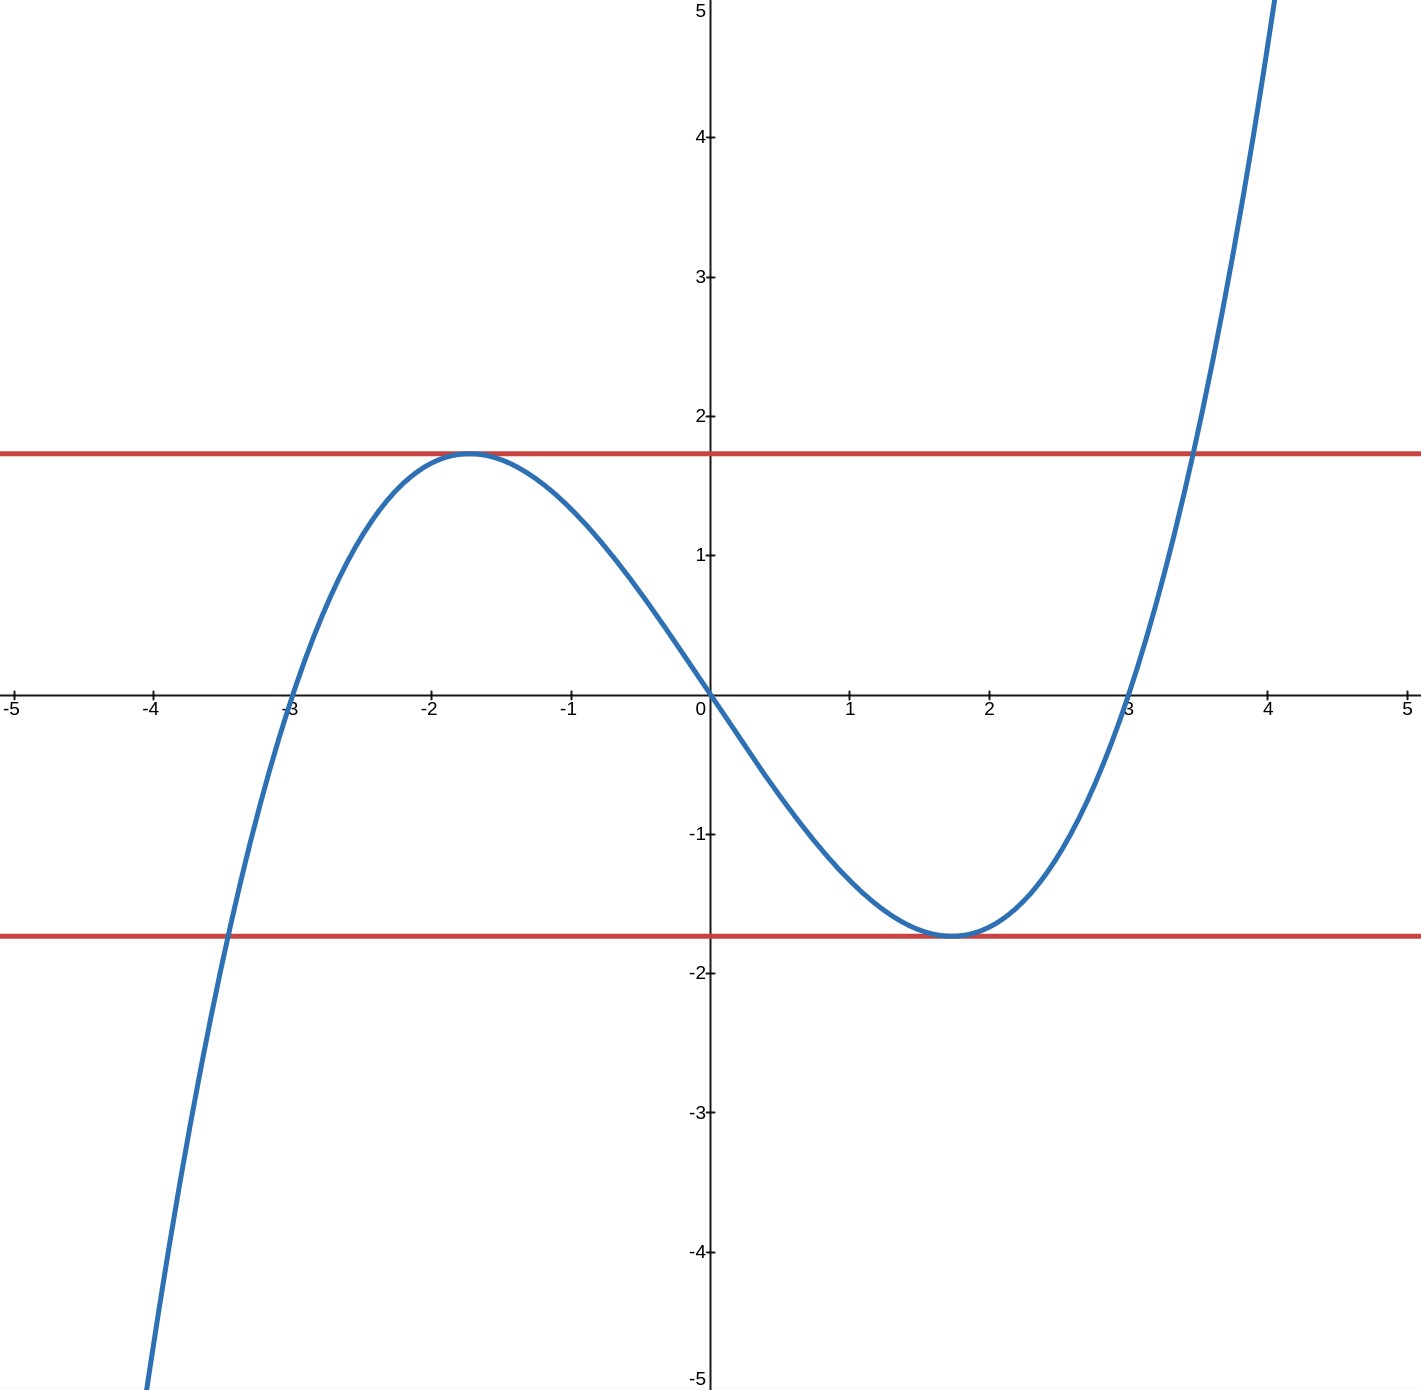
\includegraphics[width=0.3\textwidth]{figs/4-2-3b.png}
            \caption{Real Plot of $y^{2} - 3 = 0, 6y - x^{3} + 9x = 0$.}\label{fig:4-2-3b_plot}
          \end{figure}
    \item Using SageMath, we see that a monomial basis of $k[x, y] / I$ is given by $\set{1, x, y, x^{2}, xy, x^{2}y}$.
          Using this basis, $m_{x}$ has the following matrix
          \[
          \begin{pmatrix}
            0 & 0 & 0 & 0 & 0 & 18 \\
            1 & 0 & 0 & 9 & 0 & 0 \\
            0 & 0 & 0 & 6 & 0 & 0 \\
            0 & 1 & 0 & 0 & 0 & 0 \\
            0 & 0 & 1 & 0 & 0 & 9 \\
            0 & 0 & 0 & 0 & 1 & 0 \\
          \end{pmatrix}
          \]
          which has characteristic polynomial
          \[
            u^{6} - 18u^{4} + 81u^{2} - 108 = (u^{2} - 12)(u^{2} - 3)^{2}.
          \]
    \clearpage
    \item Further factoring of the characteristic polynomial over $k$ into linear parts yields that
          \[
            u^{6} - 18u^{4} + 81u^{2} - 108 = (u^{2} - 12)(u^{2} - 3)^{2} = (u - 2\sqrt{3})(u + 2\sqrt{3})(u - \sqrt{3})^{2}(u + \sqrt{3})^{2}.
          \]
          Applying~\cite[\S 4.2, Proposition 2.7]{book:UAG} yields that the points with $x$-coordinate $\pm \sqrt{3}$ each have multiplicity $2$, as expected from \Cref{fig:4-2-3b_plot}, and the other points with $x$-coordinate $\pm 2\sqrt{3}$ each have multiplicity $2$.
    \item \quest{TODO: Return once you have learned more about resultants.}
  \end{enumerate}
\end{sol}

\begin{sol}[\cite{book:UAG} Ex. 4.2.6]\label{ex:UAG_4.2.6}
  To show that $k[\overline{x}]_{M} / I k[\overline{x}]_{M}$ is a local ring, it suffices to show that $(k[\overline{x}] / I k[\overline{x}])_{M} \simeq k[\overline{x}]_{M} / I k[\overline{x}]_{M}$.
  Consider the following morphism:
  \begin{align*}
    \phi\colon k[\overline{x}]_{M} / I k[\overline{x}]_{M} &\to  (k[\overline{x}] / I k[\overline{x}])_{M} \\
                       \frac{f}{g} + I k[\overline{x}]_{M} &\mapsto \frac{f + I}{g + I}.
  \end{align*}
  It is immediate that $\phi$ is well defined and surjective.
  To see that $\phi$ is injective, suppose that $\frac{f}{g} + Ik[\overline{x}]_{M} \in \ker \phi$.
  Then $\frac{f + I}{g + I} = 0$ implies that $f \in I$.
  Thus, $f \in I k[\overline{x}]_{M}$ which implies that $\frac{f}{g} + I k[\overline{x}]_{M} = 0$.
  Thus, $\phi$ is an isomorphism which implies that $k[\overline{x}]_{M} / I k[\overline{x}]_{M}$ is a local ring.

  To see that $k[\overline{x}]_{M} / I k[\overline{x}]_{M}$ has dimension $\geq 1$ as a $k$-vector-space, we show that evaluation at $p$, $\evaluation_{p}$ is a well-defined linear surjection of vector spaces.
  It is immediate that $\evaluation_{p}$ is a linear map.
  To see that it is well defined, suppose $\frac{f}{g} + I k[\overline{x}]_{M} = \frac{f'}{g'} + I k[\overline{x}]_{M}$.
  Then we have that $\frac{fg' - f'g}{gg'} \in Ik[\overline{x}]_{M}$ which implies that $fg' - f'g \in K$.
  Thus, $\evaluation_{p}\pqty{\frac{f}{g} - \frac{f'}{g'} + I k[\overline{x}]_{M}} = 0$ and so by linearity of $\evaluation_{p}$, we have that $\evaluation_{p}\pqty{\frac{f}{g} + I k[\overline{x}]_{M}} = \evaluation_{p}\pqty{\frac{f'}{g'} + I k[\overline{x}]_{M}}$ as desired.
  Since $\evaluation_{p}$ is obviously surjective, we must have that $\dim_{k}k[\overline{x}]_{M} / I k[\overline{x}]_{M} \geq 1$.
\end{sol}

\begin{sol}[\cite{book:UAG} Ex. 4.2.7]\label{ex:UAG_4.2.7}
  As $\bigcap_{i = 1}^{n} M_{i}$ is an ideal, it is finitely generated by polynomials $\set{f_{1}, \ldots, f_{s}}$.
  For each $f_{j} \in \bigcap_{i = 1}^{n} M_{i}$, we have that for all $1 \leq i \leq n$ that $f_{j}(p_{i}) = 0$.
  Thus, $f_{j} \in \I(\V(I)) = \sqrt{I}$ and so there exists $d_{j} > 0$ such that $f^{d_{j}} \in I$.
  Let $d = \sum_{j = 1}^{s} d_{j}$.
  Then for all $f \in \bigcap_{i = 1}^{n} M_{i}$, we have that $f^{d} \in I$ and so $\pqty{\bigcap_{i = 1}^{n} M_{i}}^{d} \subseteq I$.
\end{sol}

\begin{sol}[\cite{book:UAG} Ex. 4.2.9]\label{ex:UAG_4.2.9}
  Fix $1 \leq i \leq n$.
  As $\sum_{j = 1}^{m} e_{j} \equiv 1 \pmod{I}$ and for $i \neq j$ we have that $e_{i}e_{j} \equiv 0 \pmod{I}$, we have that
  \[
    e_{i} \equiv e_{i} \sum_{j = 1}^{m} e_{j} = e_{i}^{2} + \sum_{\substack{j = 1 \\ j \neq i}}^{m} e_{i}e_{j} \equiv e_{i}^{2} \pmod{I}.
  \]
\end{sol}

\clearpage

\begin{sol}[\cite{book:UAG} Ex. 4.2.11]\label{ex:UAG_4.2.11}
  \begin{enumerate}
    \item If $f \in I$, then $f(p_{i}) = 0$ and so $[f]_{i} = [0]_{i}$ in $A_{i}$ meaning $f \in Q_{i}$.
          To see the desired description of $Q_{i}$, we have that
          \begin{align*}
            f \in Q_{i} &\iff [f]_{i} = [0]_{i} \\
                        &\iff f \in I \mathcal{O}_{i} \\
                        &\iff f = \frac{g_{i}}{u}, u \in k[\overline{x}] \setminus M_{i}, g_{i} \in I \iff f \cdot u = g_{i} \in I.
          \end{align*}
    \item Fix $1 \leq i \leq m$ and $j \neq i$.
          Let $\tilde{u} \defeq 1 - g_{j}$.
          We have that $\tilde{u} \notin M_{i}$.
          For $k \neq j$ we have that $(\tilde{u} \cdot g_{j})(p_{k}) = \tilde{u}(p_{k}) \cdot g_{j}(p_{k}) = 1 \cdot 0 = 0$.
          On the other hand, we have that $(\tilde{u} \cdot g_{j})(p_{j}) = \tilde{u}(p_{j}) \cdot g_{j}(p_{j}) = 0 \cdot 1 = 0$.
          Thus, $\tilde{u} \cdot g_{j} \in \I(\V(I)) = \sqrt{I}$ and so there exists $d$ such that $(\tilde{u} \cdot g_{j})^{d} \in I$.
          Let $u = \tilde{u}^{d}$.
          Then $u \notin M_{i} \implies \tilde{u} \notin M_{i}$ and yet $u \cdot g_{j}^{d} \in I$.
          Thus, by \textbf{(a)} we have that $g_{j}^{d} \in Q_{i}$.
    \item Since $I \subseteq Q_{i}$, we have that $\V(Q_{i}) \subseteq \set{p_{1}, \ldots, p_{m}}$ and so we can consider this finite list of points individually.
          For all $j \neq i$, there exists $d_{j}$ such that $g_{j}^{d_{j}} \in Q_{i}$.
          Since $g_{j}^{d_{j}}(p_{j}) = 1$, we have that $p_{j} \notin Q_{i}$.
          For $f \in Q_{i}$, there exists $u \notin M_{i}$ such that $u \cdot f \in I$.
          Since $u(p_{i}) \neq 0$ but $u(p_{i}) \cdot f(p_{i}) = 0$, we must have that $f(p_{i}) = 0$.
          Thus, $\V(Q_{i}) = \set{p_{i}}$.
          With this, $\sqrt{Q_{i}} = \I(\V(Q_{i})) = \I(\set{p_{i}}) = M_{i}$ as desired.
    \item Suppose that $f \cdot g \in Q_{i}$.
          If $f \in Q_{i}$ we are done, so suppose not.
          Then $f(p_{i}) \neq 0$ but $f(p_{i}) \cdot g(p_{i}) = 0$ which implies that $g(p_{i}) = 0$.
          Thus, $g \in M_{i} = \sqrt{Q_{i}}$ and so there exists $d > 0$ such that $g^{d} \in M_{i}$.
          \quest{Unsure about the relevance of the hint saying that $A_{i}$ is a local ring.}
    \item By \textbf{(a)}, we have that $I \subseteq Q_{i}$ for all $i$ and so $I \subseteq Q_{1} \cap \cdots \cap Q_{m}$.
          Now suppose that $f \in Q_{1} \cap \cdots \cap Q_{m}$ which implies that for all $i$, $f \in \ker \varphi_{i}$.
          By the proof of~\cite[\S 4.2, Theorem 2.2]{book:UAG}, this means that $f \in I$.
          Thus, $I = Q_{1} \cap \cdots \cap Q_{m}$.
    \item We know that $\varphi\colon k[\overline{x}] \to A_{1} \times \cdots \times A_{m}$ is surjective.
          Trivially, the projection $\pi_{i}\colon A_{1} \times \cdots \times A_{m} \to A_{i}$ is also surjective.
          Thus, $\varphi_{i} = \pi_{i} \circ \varphi$ is surjective.
          By an isomorphism theorem, this means that $k[\overline{x}] / Q_{i} \simeq A_{i}$.
  \end{enumerate}
\end{sol}

\begin{sol}[\cite{book:UAG} Ex. 4.2.12]\label{ex:UAG_4.2.12}
  \begin{enumerate}
    \item As $f(p_{i})$ is the only eigenvalue of $m_{f}\colon A_{i} \to A_{i}$ and every vector space is the direct sum of generalized eigenspaces for each eigenvalue of a linear map, we must have that $A_{i}$ is the only generalized eigenspace for $m_{f}$.
    \item By~\cite[\S 2.4, Theorem 4.5]{book:UAG}, the values of $f$ on $\V(I) = \set{p_{1}, \ldots, p_{m}}$ are all eigenvalues of $f$.
          The result is immediate by the uniqueness of the set of eigenvalues of a function and the consequent uniqueness of direct sum decomposition of $A$ into generalized eigenspaces.
  \end{enumerate}
\end{sol}

\begin{sol}[\cite{book:UAG} Ex. 4.2.14]\label{ex:UAG_4.2.14}
  \quest{TODO: Come back after learning more about resultants.}
\end{sol}

\begin{sol}[\cite{book:UAG} Ex. 4.2.15]\label{ex:UAG_4.2.15}
  \begin{enumerate}
    \item Let $I = \I(\ell_{1}, \ldots, \ell_{n})$.
          Since $\V(\ell_{1}, \ldots, \ell_{n}) = \set{\overline{0}}$, we must have that the matrix with rows given by the coefficients of the $\ell_{i}$ is full rank.
          Thus, $k[\overline{x}] / I \simeq k$.
          Let $f = 1$ so that $m_{f}$ is the $1 \times 1$ identity matrix.
          Then $(-1)^{1} (u - 1)^{m(\overline{0})} = \det(m_{f} - uI) = 1 - u$ which implies that $m(\overline{0}) = 1$ as desired.
    \item By~\cite[\S 4.2, Proposition 2.11]{book:UAG}, we have that the multiplicity of the origin in $\V(I)$ is also given by $\dim_{k} k[[\overline{x}]] / Ik[[\overline{x}]]$.
          Since the Jacobian matrix is invertible, \quest{there is} an automorphism of $k[[\overline{x}]]$ sending $f_{i}$ to $x_{i}$.
          Since $\overline{0} \in \V(x_{1}, \ldots, x_{n})$ which is a variety defined by homogeneous linear polynomials, by \textbf{(a)} we have that the multiplicity of the origin is $1$.

          \textbf{Remark:} Supposedly, one way to see this is via Nakayama's Lemma.
          From the \href{https://en.wikipedia.org/wiki/Nakayama%27s_lemma#Local_rings}{Wikipedia page stating an application to local rings}, we see that Nakayama's Lemma tells us that generators of the cotangent space $\mathfrak{m} / \mathfrak{m}^{2}$ lift to generators of $\mathfrak{m}$ for any maximal ideal $\mathfrak{m}$.
  \end{enumerate}
\end{sol}

\begin{sol}[\cite{book:UAG} Ex. 4.2.16]\label{ex:UAG_4.2.16}
  Let $f \in k[\overline{x}]$ be such that $f$ has an ordinary double point at the origin.
  By~\cite[\S 4.2, Proposition 2.11]{book:UAG}, the Milnor number of $0$ is given by the multiplicity of $0$ of $\ideal{\frac{\partial f}{\partial x_{1}}, \ldots, \frac{\partial f}{\partial x_{n}}}$.
  Letting $g_{i} \defeq \frac{\partial f}{\partial x_{i}}$, the Jacobian of $g_{1}, \ldots, g_{n}$ is the invertible matrix of second-order partial derivatives.
  By \Cref{ex:UAG_4.2.15}, we know this value is $1$.
  Thus, the Milnor number of an ordinary double point is $1$.
\end{sol}

\clearpage

\section{Term Orders and Division in Local Rings}

\begin{sol}[\cite{book:UAG} Ex. 4.3.8]\label{ex:UAG_4.3.8}
  \begin{enumerate}
    \item Following the given hint, let $>_{r}$ be the reverse ordering of $>$.
          Then by~\cite[\S 2.4, Corollary 6]{book:IVA}, to prove that $>_{r}$ is a well-ordering it suffices to show that $\alpha \geq_{r} 0$ for all $\alpha \in \Z_{\geq 0}^{n}$.
          Since for all $i$ we have that $1 > x_{i}$, we have that $x_{i} >_{r} 1$.
          Compatibility with multiplication then inductively shows that for all $\alpha \in \Z_{\geq 0}^{n}$ that $\alpha \geq_{r} 0$ and this $>_{r}$ is a well-ordering.
          Translating back to $>$, this shows that every nonempty set of monomials has a maximal element.
    \item Since every nonempty set of monomials has a maximal element by \textbf{(a)}, we can define $\mdeg,\ \lt$, and $\lc$ in the usual manner.
    \item \quest{Immediate}
    \item \quest{Immediate}
  \end{enumerate}
\end{sol}

\begin{sol}[\cite{book:UAG} Ex. 4.3.9]\label{ex:UAG_4.3.9}
  Clearly if the remainder is $0$, then the result of the normal form algorithm gives a certificate of ideal membership.
  However, the converse is not necessarily true as seen when dealing with division by sets that do not necessarily form a \Grobner\ (or as seen later, standard) basis.
  \quest{TODO: Example}
\end{sol}

\begin{sol}[\cite{book:UAG} Ex. 4.3.10]\label{ex:UAG_4.3.10}
  In the proof of correctness, we found polynomials $A_{l, j}, U_{j}$, and $H_{j}$ such that on the $j\textsuperscript{th}$ pass through the WHILE loop we had
  \[
    U_{j}F = A_{1, j}F_{1} + \cdots + A_{s, j}F_{s} + H_{j}.
  \]
  For $j = 0$, we can take $H_{0} = F$, $U_{0} = 1$, and $A_{l, 0} = 0$ for all $l$.
  The proof of correctness of~\cite[\S 4.2, Theorem 3.10]{book:UAG}, there are given rules on how to update not just $H_{j}$ and $U_{j}$ but also how to find $A_{l, j + 1}$ from $A_{l, j}$ depending on what $G$ is on each given loop.
\end{sol}

\begin{sol}[\cite{book:UAG} Ex. 4.3.13]\label{ex:UAG_4.3.13}
  \quest{Is there a non-tedious non-inductive way to do this?}
\end{sol}

\begin{sol}[\cite{book:UAG} Ex. 4.3.14]\label{ex:UAG_4.3.14}
  Homogenize $f, f_{1}, \ldots, f_{s}$ to obtain $F, F_{1}, \ldots, F_{s}$.
  Then run the algorithm described in~\cite[\S 4.2, Theorem 3.10]{book:UAG}.
  Dehomogenize the result by setting $t = 1$.
  We know that homogenization and dehomogenization preserve leading terms and both take units to units.
  This proves~\cite[\S 4.2, Corollary 3.13]{book:UAG}.
  \quest{TODO: SageMath implementation.}
\end{sol}

\clearpage

\section{Standard Bases in Local Rings}

\begin{sol}[\cite{book:UAG} Ex. 4.4.1]\label{ex:UAG_4.4.1}
  \begin{enumerate}
    \item Recall that every semigroup order $>$ on $R$ can be lifted to a monomial order $>'$ on $k[t, \overline{x}]$ such that homogenization and dehomogenization with respect to $t$ maintains leading terms.
          Thus, we can consider $\ideal{\lt(I)} \subseteq k[t, \overline{x}]$ with respect to $>'$.
          Here, as we are dealing with a monomial order, Dickson's Lemma implies that $\ideal{\lt(I)}$ has a finite generating set.
          As dehomogenization, by setting $t = 1$, takes leading terms to leading terms, we have that $\ideal{\lt(I)} \subseteq R$ has a finite generating set.
    \item \quest{Immediate}
  \end{enumerate}
\end{sol}

\begin{sol}[\cite{book:UAG} Ex. 4.4.2]\label{ex:UAG_4.4.2}
  \begin{enumerate}
    \item Clearly if the remainder of $f$ on division by $G$ is $0$ and $\ideal{G} = I$ then $f \in I$.
          Now suppose that $f \in I$.
          Then $f = f + 0$ and the uniqueness of the remainder as shown in~\cite[\S 4.4, Theorem 4.3]{book:UAG} shows that the remainder upon division by $G$ is $0$.
    \item We saw in \nameref{ex:UAG_4.4.1} that every local ring $R$ has a standard basis which is finite.
          \quest{Unsure where the above part is used.}
    \item \quest{Trivial}
  \end{enumerate}
\end{sol}

\begin{sol}[\cite{book:UAG} Ex. 4.4.3]\label{ex:UAG_4.4.3}
  \quest{TODO}
\end{sol}

\begin{sol}[\cite{book:UAG} Ex. 4.4.4]\label{ex:UAG_4.4.4}
  \quest{TODO}
\end{sol}

\begin{sol}[\cite{book:UAG} Ex. 4.4.6]\label{ex:UAG_4.4.6}
  The algorithm is basically the one given in the proof of $c \implies a$ in the proof of~\cite[\S 4.4, Theorem 4.3]{book:UAG}.
  \quest{TODO: SageMath implementation.}
\end{sol}

\clearpage

\section{Applications of Standard Bases}

\begin{sol}[\cite{book:UAG} Ex. 4.5.2]\label{ex:UAG_4.5.2}
  \begin{enumerate}
    \item As $f_{1}, \ldots, f_{n}$ are homogeneous already, homogenization with respect to $x_{0}$ does nothing.
          Thus, as $\V(f_{1}, \ldots, f_{n}) = \set{\overline{0}}$, the have no non-trivial solutions when $x_{0} = 0$.
          Given this, \Bezout's Theorem~\cite[\S 3.5, Theorem 5.5]{book:UAG} applies.
          Combining \Bezout's Theorem with~\cite[\S 4.2, Theorem 2.5]{book:UAG} yields that $d_{1} \cdots d_{n} = \dim k[\overline{x}] / I = m(\overline{0})$.
    \item Apply \textbf{(a)} to $\ideal{\frac{\partial f}{\partial x_{1}}, \ldots, \frac{\partial f}{\partial x_{n}}}$.
  \end{enumerate}
\end{sol}

\begin{sol}[\cite{book:UAG} Ex. 4.5.3]\label{ex:UAG_4.5.3}
  \quest{TODO after installing Singular}
\end{sol}

\begin{sol}[\cite{book:UAG} Ex. 4.5.4]\label{ex:UAG_4.5.4}
  \quest{TODO after installing Singular}
\end{sol}

\begin{sol}[\cite{book:UAG} Ex. 4.5.5]\label{ex:UAG_4.5.5}
  \begin{enumerate}
    \item Trivial.
    \item We take ideas from~\cite[Proposition 4]{Mora1989}.
          Recall that degree-anticompatible orderings are local orderings.
          Then for all $h = \frac{f}{1 + g} \in k[\overline{x}]_{\ideal{x_{1}, \ldots, x_{n}}}$ we have that $\lt(h) = \lt(f) = \lt(f_{\min}) = \lt(h_{\min})$.
          Let $\mathrm{in}(I) = \ideal{f_{\min} \mid f \in I}$.
          Let $G = \set{g_{1}, \ldots, g_{t}}$.
          By similar arguments to \textbf{(a)}, we have that
          \[
            \ideal{\lt(\mathrm{in}(I))} = \ideal{\lt(I)} = \ideal{\lt(G)} = \ideal{\lt(\mathrm{in}(G))}.
          \]
          Thus, $\mathrm{in}(G)$ is a standard basis for $\mathrm{I}$ and so $\mathbf{C}(V) = \V(\mathrm{in}(G))$.

          \textbf{Remark:} In fact, we have shown more.
          We know that $G = \set{g_{1}, \ldots, g_{t}}$ are all polynomials and so it makes sense to talk about \Grobner\ bases.
          Let $>$ be the degree-anticompatible ordering in question and define $>_{w}$ by undoing the degree-anticompatibility in that
          \[
            \overline{x}^{\alpha} >_{w} \overline{x}^{\beta} \iff \abs{\alpha} > \abs{\beta} \text{ or } \abs{\alpha} = \abs{\beta} \text{ and } \overline{x}^{\alpha} > \overline{x}^{\beta}.
          \]
          Then we can actually show that $G$ is a \Grobner\ basis with respect to $>_{w}$.
    \item \quest{TODO after installing Singular}
  \end{enumerate}
\end{sol}

\chapter{Modules}

\section{Modules over Rings}

\quest{TODO: Every exercise as qualifying prep.}

\begin{sol}[\cite{book:UAG} Ex. 5.1.2]\label{ex:UAG_5.1.2}
  \begin{enumerate}
    \item Clearly $f_{1}, f_{2}, f_{3} \in \ker A$ and so $M \subseteq \ker A$.
          Now suppose that $f = \begin{pmatrix} p & q & r \end{pmatrix}^{\top} \in R^{3}$ such that $Af = 0$.
          Thus, $xp + yq + zr = 0$.
          As $k[x, y, z] = k[x, y][z]$, there exists $p_{1}, q_{1} \in k[x, y]$ and $p_{2}, q_{2} \in k[x, y, z]$ such that $p = p_{1} + z p_{2}$ and $q = q_{1} + z q_{2}$.
          Let $z = 0$.
          Then $0 = x p_{1} + y q_{1}$ and so there exists $a \in k[x, y]$ such that $xa = q_{1}$ and so $-ya = p_{1}$.
          Given this, we have that
          \[
          \begin{pmatrix}
            p \\ q \\ r
          \end{pmatrix}
          =
          -a f_{1} +
          \begin{pmatrix}
            z p_{2} \\ z q_{2} \\ r
          \end{pmatrix}.
          \]
          As both $\begin{pmatrix} p & q & r \end{pmatrix}^{\top}$ and $-a f_{1}$ are in $\ker A$, we have that $\begin{pmatrix} z p_{2} & z q_{2} & r \end{pmatrix}^{\top}$ is in $\ker A$.
          Thus, $xzp_{2} + yzq_{2} + zr = 0$ and so $r = -xp_{2} - y q_{2}$ and overall we have that
          \[
          \begin{pmatrix}
            p \\ q \\ r
          \end{pmatrix}
          =
          -a f_{1} +
          \begin{pmatrix}
            z p_{2} \\ z q_{2} \\ r
          \end{pmatrix}
          = -a f_{1} + p_{2} f_{2} + q_{2} f_{3} \in M.
          \]
    \item Consider $\gen{f_{1}, f_{2}}$.
          Then for all $a, b \in k[x, y]$ we have that $a f_{1} + b f_{2} = \begin{pmatrix} a y + b z & -a x & - b x \end{pmatrix}^{\top}$.
          Thus, for all $\begin{pmatrix} p & q & r \end{pmatrix}^{\top} \in \gen{f_{1}, f_{2}}$ we must have that $x \mid q$ and $x \mid r$.
          However, we know that $f_{3} = \begin{pmatrix} 0 & z & -y \end{pmatrix}^{\top} \in M$ but $x \nmid z$ and $x \nmid -y$.
          Thus, $\gen{f_{1}, f_{2}} \subsetneq M$.
          The other cases are similar.

          \clearpage

    \item We have that $-z f_{1} + y f_{2} - x f_{3} = \overline{0}$.
    \item Nothing to do.
    \item We pass to $F = \mathrm{Frac}(R)$.
          Here we see that $M$ has dimension $\leq 2$ as a $F$ vector space by \textbf{(c)}.
          Clearing denominators of any $F$-linear dependence yields an $R$-linear dependence of 3 vectors and so there is no linearly independent set with 3 vectors.
          \quest{TODO: brutal calculuation}
  \end{enumerate}
\end{sol}

\begin{sol}[\cite{book:UAG} Ex. 5.1.8]\label{ex:UAG_5.1.8}
  \begin{enumerate}
    \item Let $\phi\colon M \to R$ be a $R$-module homomorphism such that $\phi(x^{2}) = y$ and $\phi(y^{3}) = x$.
          Then we must have that
          \[
            0 = \phi(0) = \phi(y^{3}x^{2} - x^{2}y^{3}) = y^{3} \phi(x^{2}) - x^{2} \phi(y^{3}) = y^{4} - x^{3}.
          \]
          However, $y^{4} \neq x^{3}$ yields a contradiction and so no such $\phi$ exists.
    \item Let $\phi\colon M \to R$ be a $R$-module homomorphism and let $a = \phi(x^{2})$ and $b = \phi(y^{3})$.
          Then as above, we must have that $y^{3}a = x^{2} b$.
          This means that $y^{3} \mid b$ and so there exists $c \in k[x, y]$ such that $y^{3} c = b$.
          Then $y^{3} a = x^{2} b = x^{2} y^{3} c$ implies that $a = x^{2} c$.
          So $\phi(x^{2}) = x^{2} c$ and $\phi(y^{3}) = y^{3} c$, \ie\ $\phi(1) = c$.
          This implies that $\Hom(\gen{x^{2}, y^{3}}, k[x, y]) \simeq k[x, y]$ as $k[x, y]$-modules as we can choose any $c$ and such $c$ is unique.
  \end{enumerate}
\end{sol}

\begin{sol}[\cite{book:UAG} Ex. 5.1.9]\label{ex:UAG_5.1.9}
  \begin{enumerate}
    \item Follows immediately from \quest{Exercise 1.}
    \item Clearly $\gen{f_{1}, f_{2}} \subseteq M$.
          Now let $(X_{1}, X_{2}, X_{3}) \in M$.
          Thus, $X_{1} + x^{2}X_{2} + (y - 2)X_{3} = 0$ so that $X_{1} = -x^{2}X_{2} - (y - 2)X_{3}$ which immediately implies that $(X_{1}, X_{2}, X_{3}) = (-x^{2}X_{2} - (y - 2)X_{3}, X_{2}, X_{3})$.
          This means that $(X_{1}, X_{2}, X_{2}) \in \gen{f_{1}, f_{2}}$ and so $\gen{f_{1}, f_{2}} = M$ as desired.
    \item \quest{Strightforward genearlization of above argument.}
  \end{enumerate}
\end{sol}

\clearpage

\begin{sol}[\cite{book:UAG} Ex. 5.1.10]\label{ex:UAG_5.1.10}
  \begin{enumerate}
    \item We know that $\gen{a_{1}, \ldots, a_{m}} = R$ if and only if $1 \in \gen{a_{1}, \ldots, a_{m}}$.
          So we show that the morphism is surjective if and only if $1 \in \gen{a_{1}, \ldots, a_{m}}$.
          If the morphism is surjective, then there exists $f = \begin{pmatrix} f_{1} & \cdots & f_{m} \end{pmatrix}^{\top}$ such that $a_{1}f_{1} + \cdots + a_{m}f_{m} = 1$ and so $1 \in \gen{a_{1}, \ldots, a_{m}}$.
          Now suppose that $1 \in \gen{a_{1}, \ldots, a_{m}}$.
          Choose $g_{1}, \ldots, g_{m} \in R$ such that $1 = a_{1}g_{1} + \cdots + a_{m}g_{m}$.
          Let $r \in R$.
          Define $f_{i} = f g_{i}$ for $1 \leq i \leq m$.
          Then clearly for $f = \begin{pmatrix} f_{1} & \cdots & f_{m} \end{pmatrix}^{\top}$ we have that $f$ maps to $g$ and so the morphism is onto.
    \item This follows from the fact that nonzero constants in $k[\overline{x}]$ are invertible.
    \item We have that
          \[
            \frac{1}{2}(x + xy) + \pqty{-\frac{x}{2} + 1}(1 - y) + (-y)(1 + x) = 1.
          \]
    \item \quest{Gave up.}
    \item We see that $a_{3} h_{1} - a_{2} h_{2} + a_{1} h_{3} = 0$ showing a linear dependence.
          Consider $\gen{h_{1}, h_{2}}$.
          Notice that for every $\begin{pmatrix} X_{1} & X_{2} & X_{3} \end{pmatrix}^{\top} \in \gen{h_{1}, h_{2}}$ we must have that $a_{1} \mid X_{2}$ and $a_{2} \mid X_{3}$.
          Clearly this is not true for $h_{3}$ and so $h_{3} \notin \gen{h_{1}, h_{2}}$ and so $\gen{h_{1}, h_{2}} \neq M$.
          Showing $\gen{h_{1}, h_{3}}, \gen{h_{2}, h_{3}} \neq M$ is similar.
  \end{enumerate}
\end{sol}

\begin{sol}[\cite{book:UAG} Ex. 5.1.11]\label{ex:UAG_5.1.11}
  We have that
  \begin{align*}
    3f_{1} + 2f_{2} + 2f_{3} &= 3f_{1} + (1 + x)f_{2} + (1 - x)f_{2} + 2f_{3} \\
                             &= (1 - x)f_{2} + 2f_{3} \\
                             &= \frac{1}{2}((2 - x)f_{2} + 4f_{3}) \\
                             &= \frac{1}{2} \cdot 0 = 0.
  \end{align*}
\end{sol}

\begin{sol}[\cite{book:UAG} Ex. 5.1.17]\label{ex:UAG_5.1.17}
  We saw in \Cref{ex:UAG_5.1.2}(c) that  $\Syz(f_{1}, f_{2}, f_{3}) = \gen{\begin{pmatrix} -z & y & -x \end{pmatrix}}$.
  Since $M = \gen{f_{1}, f_{2}, g_{3}}$ has 3 generators and $\Syz(f_{1}, f_{2}, f_{3})$ has one generator, we have that our presentation matrix $A$ is $3 times 1$.
  Then, $\varphi\colon M \to R^{l}$ is given by an $l \times 3$ matrix $B = (b_{i, j})$.
  The condition from~\cite[\S 5.1, Proposition 1.11]{book:UAG} stating that $BA = 0$ means that for all $1 \leq i \leq l$ we have that $-z b_{i, 1} + y b_{i, 2} - x b_{i, 3} = 0$.
  This completely characterizes all morphisms $\varphi\colon M \to R^{l}$.
\end{sol}

\clearpage

\begin{sol}[\cite{book:UAG} Ex. 5.1.18]\label{ex:UAG_5.1.18}
  Let $c = \begin{pmatrix} c_{1} & \cdots & c_{l} \end{pmatrix}$ and $d = \begin{pmatrix} d_{1} & \cdots & d_{l} \end{pmatrix}$.
  Suppose that $\sum_{i = 1}^{l} c_{i}f_{i} = \sum_{i = 1}^{l} d_{i}f_{i}$.
  We have that $\sum_{i = 1}^{l} c_{i}\varphi(f_{i}) = Bc$ and $\sum_{i = 1}^{l} d_{i}\varphi(f_{i}) = Bd$.
  Showing that $\varphi$ is well-defined is equivalent to showing that $Bc = Bd$ for all $c, d$.
  Equivalently, we want to show that $Bx = 0$ for all $x \in \Syz(f_{1}, \ldots, f_{l})$.
  Recall that the columns of $A$ are the generators of $\Syz(f_{1}, \ldots, f_{n})$,
  Thus, $\varphi$ is well-defined if and only if $BA = 0$.
\end{sol}

\begin{sol}[\cite{book:UAG} Ex. 5.1.19]\label{ex:UAG_5.1.19}
  \begin{enumerate}
    \item Let $c = \begin{pmatrix} c_{1} & \cdots & c_{s} \end{pmatrix}$.
          If $\sum_{i = 1}^{s} c_{i}f_{i} = 0$, then $Ac = 0$.
          But $A$ is invertible and so $c = 0$ meaning that $\set{f_{1}, \ldots, f_{s}}$ forms a basis.
    \item Suppose that $N \simeq R^{s}$.
          Then there exists an isomorphism $\varphi\colon N \to R^{s}$.
          This is given by a matrix $A$ where $A$ is invertible as $\varphi$ is an isomorphism.
          We have a standard basis $\set{e_{1}, \ldots, e_{s}}$ for $R^{s}$.
          Define $f_{i}$ as in \textbf{(a)}.
          We saw that this forms a basis for $N$ and so $N$ is free.

          Now suppose that $N$ is free with basis $\set{f_{1}, \ldots, f_{s}}$.
          Let $\varphi\colon N \to R^{s}$ be given by $f_{i} \mapsto e_{i}$ and extend by linearity.
          This is well defined, linear, surjective, and injective by linear independence of the basis $\set{e_{1}, \ldots, e_{s}}$.
          Thus, $N \simeq R^{s}$.
  \end{enumerate}
\end{sol}

\clearpage

\section{Monomial Orders and \Grobner\ Bases for Modules}

\begin{sol}[\cite{book:UAG} Ex. 5.2.6]\label{ex:UAG_5.2.6}
  \begin{enumerate}
    \item Follows immediately from the distributivity of multiplication in $S = k[x_{1}, \ldots, x_{n}, X_{1}, \ldots, X_{m}]$.
    \item Follows immediately from the distributivity of multiplication in $S$ and the fact that $R = k[x_{1}, \ldots, x_{n}]$ contains no monomials containing any of the $X_{j}$.
    \item Consider $f_{i}$, one of the generators of $M$.
          Then there exists $r_{i} \in R$ such that $f_{i} = \sum_{i = 1}^{s} r_{i} e_{i}$.
          We have that $F_{i} = \varphi(f_{i}) = \sum_{i = 1}^{s} r_{i} X_{i}$ and so each $F_{i}$ is an element of $S_{1}$.
          By $R$-linearity, this shows that $\varphi(M) \subseteq \ideal{F_{1}, \ldots, F_{s}}S \cap S_{1}$.
          Now suppose that $f \in \ideal{F_{1}, \ldots, F_{s}}S \cap S_{1}$.
          Then as $f \in \ideal{F_{1}, \ldots, F_{s}}S$, there exists $r_{i} \in S$ such that $f = \sum_{i = 1}^{s} r_{i}F_{i}$.
          Note that each $F_{i} \in S_{1}$.
          Thus, as polynomial rings over a field are a domain and $f \in S_{1}$, we must have that each $r_{i} \in R$ instead of just $r_{i} \in S$.
          Thus, $f = \varphi\pqty{\sum_{i = 1}^{s} r_{i} f_{i}}$ as desired.
    \item The fact that the given modification of Buchberger's Algorithm works follows from the fact that in \textbf{(c)}, we know that the image of $M$ in $S$ under $\varphi$ is contained in $S_{1}$ and so any other $S$-polynomials not in $S_{1}$ are irrelevant as they do not appear in the image of $M$.
  \end{enumerate}
\end{sol}

\begin{sol}[\cite{book:UAG} Ex. 5.2.7]\label{ex:UAG_5.2.7}
  Recall that the only monomial ordering on $R = k[x]$ is $1 < x < x^{2} < \cdots$.
  Let $M$ be some submodule of $R^{m}$ and $G$ a \Grobner\ basis for $M$.
  Without loss of generality, say $G$ is monic and reduced.
  Suppose there were elements of $G$ whose leading terms both contain some $e_{i}$, say $x^{a}e_{i}$ and $x^{b}e_{i}$.
  Then either $x^{a} \mid x^{b}$ or $x^{b} \mid x^{a}$.
  So $G$ is not reduced, a contradiction and so no such pair of elements can exist.
  Via similar logic, if an element of $G$ has a term which contains $e_{i}$, then the $i$-th component of every other element of $G$ must be zero.
  In particular, this shows that every monic, reduced \Grobner\ basis of a submodule of $R^{m}$ must have $\leq m$ elements.
  Thus, by the uniqueness of monic, reduced \Grobner\ bases, there are at most $2^{m}$ submodules of $R^{m}$.
\end{sol}

\clearpage

\section{Computing Syzygies}

\begin{sol}[\cite{book:UAG} Ex. 5.3.1]\label{ex:UAG_5.3.1}
  We have that
  \[
    \mathbf{s}_{i j} \cdot \begin{pmatrix} g_{1} & \cdots & g_{s} \end{pmatrix}^{\top} = \frac{x^{\gamma_{i j}}}{\lt(g_{i})} g_{i} - \frac{x^{\gamma_{i j}}}{\lt(g_{j})}g_{j} - \sum_{k = 1}^{s} a_{i j k} g_{k} = S(g_{i}, g_{j}) - S(g_{i}, g_{j}) = 0.
  \]
  Thus, $\mathbf{s}_{i j} \in \Syz(g_{1}, \ldots, g_{s})$.
\end{sol}

\begin{sol}[\cite{book:UAG} Ex. 5.3.7]\label{ex:UAG_5.3.7}
  Suppose $h_{0} \in I \cap J$.
  Then there exists $h_{1}, \ldots, h_{t}, h_{t + 1}, \ldots, h_{t + s}$ such that $h_{0} = \sum_{i = 1}^{t} h_{i}f_{i}$ and $h_{0} = \sum_{j = 1}^{s} h_{t + j}g_{j}$.
  Then, it is easy to see that
  \[
    \mathbf{0} = h_{0}\mathbf{v}_{0} + \sum_{i = 1}^{t} -h_{i}\mathbf{v}_{i} + \sum_{j = 1}^{s} h_{t + j}\mathbf{v}_{t + j}
  \]
  and so $\begin{pmatrix} h_{0} & h_{1} & \cdots & h_{t + s} \end{pmatrix}^{\top} \in \Syz(\mathbf{v}_{0}, \mathbf{v}_{1}, \ldots, \mathbf{v}_{t}, \mathbf{v}_{t + 1}, \ldots \mathbf{v}_{t + s}) \subseteq R^{t + s + 1}$.
\end{sol}

\begin{sol}[\cite{book:UAG} Ex. 5.3.10]\label{ex:UAG_5.3.10}
  \begin{enumerate}
    \item Recall from~\cite[\quest{Exercise 1.3.12}]{book:UAG} that if $\set{g_{1}, \ldots, g_{t}}$ is \Grobner\ basis for $I \cap \ideal{h}$ then $I \colon \ideal{h}$ has a \Grobner\ basis given by $\ideal{g_{1} / h, \ldots, g_{t} / h}$.
          Given $I = \gen{f_{1}, \ldots, f_{s}}$ and $h$, first compute the generators of the syzygy modules $\Syz(\mathbf{v}_{0}, \mathbf{v}_{1}, \ldots, \mathbf{v}_{s}, \mathbf{v}_{s + 1})$ where
          \begin{gather*}
            \mathbf{v}_{0} = \begin{pmatrix} 1 \\ 1 \end{pmatrix}, \\
            \mathbf{v}_{1} = \begin{pmatrix} f_{1} \\ 0 \end{pmatrix}, \ldots, \mathbf{v}_{s} = \begin{pmatrix} f_{1} \\ 0 \end{pmatrix}, \\
            \mathbf{v}_{s + 1} = \begin{pmatrix} 0 \\ h \end{pmatrix}.
          \end{gather*}
          By~\cite[\S 5.3, Proposition 3.11]{book:UAG}, the first components of these generators are the generators $\ideal{g_{1}, \ldots, g_{t}}$ of $I \cap \ideal{h}$.
          Furthermore, if  $\begin{pmatrix} g_{i} & h_{i, 1} & \cdots & h_{i, s} & h_{i, s + 1} \end{pmatrix}^{\top}$ is the syzygy generator witnessing $g_{i}$, then we can compute $g_{i} / h$ without division.
          To see this, study the second row of the following syzygy relation:
          \[
            \mathbf{0} = g_{i}\mathbf{v}_{0} + \mathbf{v}_{1} h_{i, 1} + \cdots \mathbf{v}_{s} h_{i, s} + \mathbf{v}_{s + 1} h_{i, s + 1}
          \]
          This means $0 = g_{i} + h \cdot h_{i, s + 1}$ and so $g_{i} / h = -h_{i, s + 1}$.
          Thus, we can recover the generators of $I \colon \ideal{h}$ without doing polynomial division.
    \item \quest{Is there anything better} than repeating~\cite[\S 5.3, Proposition 3.11]{book:UAG} multiple times?
  \end{enumerate}
\end{sol}

\begin{sol}[\cite{book:UAG} Ex. 5.3.12]\label{ex:UAG_5.3.12}
  Let $f_{1}, f_{2} \in k[\overline{x}]$ be nonzero.
  Then $\Syz(f_{1}, f_{2}) \subseteq k[\overline{x}]^{2}$ is the set of $\begin{pmatrix} a_{1} & a_{2} \end{pmatrix}^{\top}$ such that $a_{1}f_{1} + a_{2}f_{2} = 0$.
  Let $g = \gcd(f_{1}, f_{2})$ and let $g_{1} = \frac{f_{2}}{g}$ and $g_{2} = \frac{f_{1}}{g}$.
  Then it is easy to see that $\begin{pmatrix} g_{1} & -g_{2} \end{pmatrix}^{\top}$ generates $\Syz(f_{1}, f_{2})$.
  Indeed, suppose that $\begin{pmatrix} a_{1} & a_{2} \end{pmatrix}^{\top} \in \Syz(f_{1}, f_{2})$.
  Then since $a_{1}f_{1} + a_{2}f_{2} = 0$, we have that $a_{1}f_{1} = -a_{2}f_{2}$ and so $f_{2} \mid a_{1}f_{1}$.
  Thus, $g_{1} = \frac{f_{2}}{g} \mid a_{1}$.
  Similarly, we get that $g_{2} = \frac{f_{1}}{g} \mid -a_{2}$.
  Thus, $\begin{pmatrix} a_{1} & a_{2} \end{pmatrix}^{\top} \in \gen{\begin{pmatrix} g_{1} & -g_{2} \end{pmatrix}^{\top}}$.
\end{sol}

\clearpage

\section{Modules over Local Rings}

\begin{sol}[\cite{book:UAG} Ex. 5.4.1]\label{ex:UAG_5.4.1}
  From~\Cref{ex:UAG_4.1.11}, we know that every ideal in $k[x_{1}, \ldots, x_{n}]_{\ideal{x_{1}, \ldots, x_{n}}}$ is generated by a finite set of polynomials in $k[x_{1}, \ldots, x_{n}]$.
  Then the claim follows from the same proof as~\cite[\S 5.2, Proposition 2.3a]{book:UAG}.
\end{sol}

\begin{sol}[\cite{book:UAG} Ex. 5.4.4]\label{ex:UAG_5.4.4}
  \begin{enumerate}
    \item We have that $\V(M) = \set{(1, 1)} \cup \set{x = 0}$.
          Given this, we see that if we remove any generator of the ideal, the set of common zeros will then include a whole new line of common zeros, thus defining a different variety.
          This shows that if we remove any particular generator then we no longer have the ideal $M$ and so $\set{xy(y - 1), xy(x - 1), x(y - 1)(x - 1)}$ is unshortenable.
    \item Let $N = \ideal{xy^{2} - x^{2}y, x^{2} - x}$.
          We show that the generators of $N$ are in $M$ and vice versa, which implies that $M = N$:
          \begin{gather*}
            xy^{2} - x^{2}y = xy(y - 1) - xy(x - 1), \\
            x^{2} - x = -x(y - 1)(x -1) + xy(x - 1), \\
            xy(y - 1) = xy^{2} - x^{2}y + y(x^{2} - x), \\
            xy(x - 1) = y(x^{2} - x), \\
            x(y - 1)(x - 1) = (y - 1)(x^{2} -x).
          \end{gather*}
  \end{enumerate}
\end{sol}

\begin{sol}[\cite{book:UAG} Ex. 5.4.6]\label{ex:UAG_5.4.6}
  \begin{enumerate}
    \item By~\cite[\S 4.3, Proposition 3.10]{book:UAG}, there exists free $R$ modules $L$ and $L'$ such that $\Syz(f_{1}, \ldots, f_{t}) \oplus L \simeq \Syz(g_{1}, \ldots, g_{s}) \oplus L'$.
          Since $\Syz(g_{1}, \ldots, g_{s})$ and $L'$ are both free, their direct sum must also be free.
          Thus, $\Syz(f_{1}, \ldots, f_{t})$ is projective.
    \item Since $R$ is a free $R$-module, we have that $R = \ideal{1}$ and $\Syz(1) = \ideal{0}$ is free.
          Take $g_{1} = 1$.
          By \textbf{(a)}, we have that $\Syz(f_{1}, \ldots, f_{t})$ is projective.
  \end{enumerate}
\end{sol}

\chapter{Free Resolutions}

\section{Presentations and Resolutions of Modules}

\begin{sol}[\cite{book:UAG} Ex. 6.1.7]\label{ex:UAG_6.1.7}
  \begin{enumerate}
    \item Denote the kernel morphisms as $k_{i}\colon \ker(\varphi_{i}) \to M_{i}$.
          Note that the morphism $\varphi_{i}\colon M_{i} \to \ker(\varphi_{i - 1})$ is well defined as $\im(\varphi_{i}) = \ker(\varphi_{i - 1})$.
          Exactness at $\ker(\varphi_{i})$ is immediate as $k_{i}$ is an inclusion morphism and thus injective.
          To show exactness at $M_{i}$, we want to show that $\im(k_{i}) = \ker(\varphi_{i})$ which is immediate as $\im(k_{i}) = \ker(\varphi_{i})$ as the inclusion map $k_{i}$ is injective.
          Exactness at $\ker(\varphi_{i - 1})$ follows from the fact that $\ker(\varphi_{i - 1}) = \im(\varphi_{i})$ and obviously morphisms are surjective onto their images.
    \item We clearly have exactness as $\ker(\varphi_{n - 1})$ as inclusion morphisms are injective.
          Again, let $k_{n - 1}$ be the kernel morphism $k_{n - 1}\colon \ker(\varphi_{n - 1}) \to M_{n - 1}$.
          To show exactness as $M_{n - 1}$, we want that $\im(k_{i}) = \ker(\varphi_{n - 1})$ which is immediate again by the exactness of $0 \to \ker(\varphi_{n - 1}) \xrightarrow{k_{n - 1}} M_{i} \xrightarrow{\varphi_{n - 1}} N_{i} \to 0$.
          For $1 \leq i \leq n - 2$, showing exactness at $M_{i}$ amounts to showing that $\im(\varphi_{i + 1}) = \ker(\varphi_{i})$.
          This follows from exactness at $N_{i + 1} = \ker(\varphi_{i})$ in the given short exact sequences.
          Finally, exactness at $\im(\varphi_{1})$ is immediate as every morphism is surjective onto its image.
    \item Follows from the above and discussion prior to~\cite[\S 6.1, Definition 1.9]{book:UAG}.
  \end{enumerate}
\end{sol}

\printbibliography
\end{document}
